\documentclass[11pt,a4paper]{article}
\usepackage[T1]{fontenc}
\usepackage[utf8]{inputenc}
\usepackage{lmodern}
\usepackage[margin=22mm,headheight=16pt]{geometry}
\usepackage{amsmath,amssymb,graphicx,array,longtable,booktabs}
\usepackage{microtype,xcolor,hyperref,xurl,fancyhdr}
\definecolor{Navy}{HTML}{17324D}
\definecolor{Teal}{HTML}{087F8C}
\definecolor{Gold}{HTML}{B88128}
\hypersetup{colorlinks=true,linkcolor=Navy,urlcolor=Teal,bookmarksnumbered=true,hypertexnames=false}
\setlength{\parindent}{0pt}
\setlength{\parskip}{6pt}
\setlength{\emergencystretch}{4em}
\setcounter{tocdepth}{1}
\pagestyle{fancy}\fancyhf{}
\fancyfoot[R]{\small\thepage}
\fancyfoot[L]{\small\sffamily Sharif University of Technology}
\renewcommand{\headrulewidth}{0.3pt}
\makeatletter
\renewcommand\section{\@startsection{section}{1}{\z@}{-3.2ex plus -1ex minus -.2ex}{1.6ex plus .2ex}{\normalfont\Large\sffamily\bfseries\color{Navy}}}
\renewcommand\subsection{\@startsection{subsection}{2}{\z@}{-2.5ex plus -1ex minus -.2ex}{1.2ex plus .2ex}{\normalfont\large\sffamily\bfseries\color{Teal}}}
\makeatother
\fancyhead[L]{\small\sffamily\color{Navy}Reza Sanaee Nezhad}\fancyhead[R]{\small\sffamily\color{Teal}Technical Report}\begin{document}
\begin{titlepage}\centering\vspace*{7mm}

\includegraphics[width=31mm]{assets/sharif_emblem_en.png}\par\vspace{5mm}
{\Large\sffamily\bfseries\color{Navy}SHARIF UNIVERSITY OF TECHNOLOGY\par}
\vspace{2mm}{\sffamily Department of Electrical Engineering\par}
\vspace{17mm}{\color{Teal}\rule{\linewidth}{1.4pt}}\par\vspace{6mm}
{\large\sffamily\color{Teal}TECHNICAL REPORT\par}
\vspace{8mm}{\huge\sffamily\bfseries\color{Navy}Seven-Bus Power-Flow and Contingency Analysis in PowerWorld\par}
\vspace{9mm}{\color{Gold}\rule{45mm}{1pt}}\par\vfill
\begin{minipage}{.88\linewidth}{\sffamily\color{Teal}AUTHOR}\par{\Large\sffamily Reza Sanaee Nezhad}\par Student ID: 401101502\par\vspace{7mm}
{\sffamily\color{Teal}INSTRUCTOR / INSTRUCTORS}\par
Instructor not stated in supplied assignment\par\vspace{7mm}
{\sffamily\color{Teal}ACADEMIC CONTEXT}\par
Energy Systems Analysis\par\end{minipage}\vfill
\end{titlepage}
\tableofcontents\clearpage
\section{Attribution and study scope}

The submitted project is attributed to Ashkan Yousefnia (401102829) and Reza Sanaee Nezhad (401101502). The source does not identify separate individual contributions. A PowerWorld case studies two iterative solvers, reactive compensation, tap adjustment, parallel equipment, load shedding, and three contingencies. All 27 experiment report pages and their simulator tables/\allowbreak{}screenshots are retained;\allowbreak{} this edition translates the Persian portions and expands the technical interpretation of the English portions.

\section{Gauss-Seidel iteration}

The report records a single-iteration view, a run allowing 100 iterations, running status, bus-flow listing, and bus mismatch listing. A maximum-iteration setting is not the same as a measured convergence count. Assess convergence from the reported residuals and solver status. The screenshots are preserved so the actual simulator state remains inspectable rather than replaced by a generic claim of success.

\begin{figure}[!htbp]\centering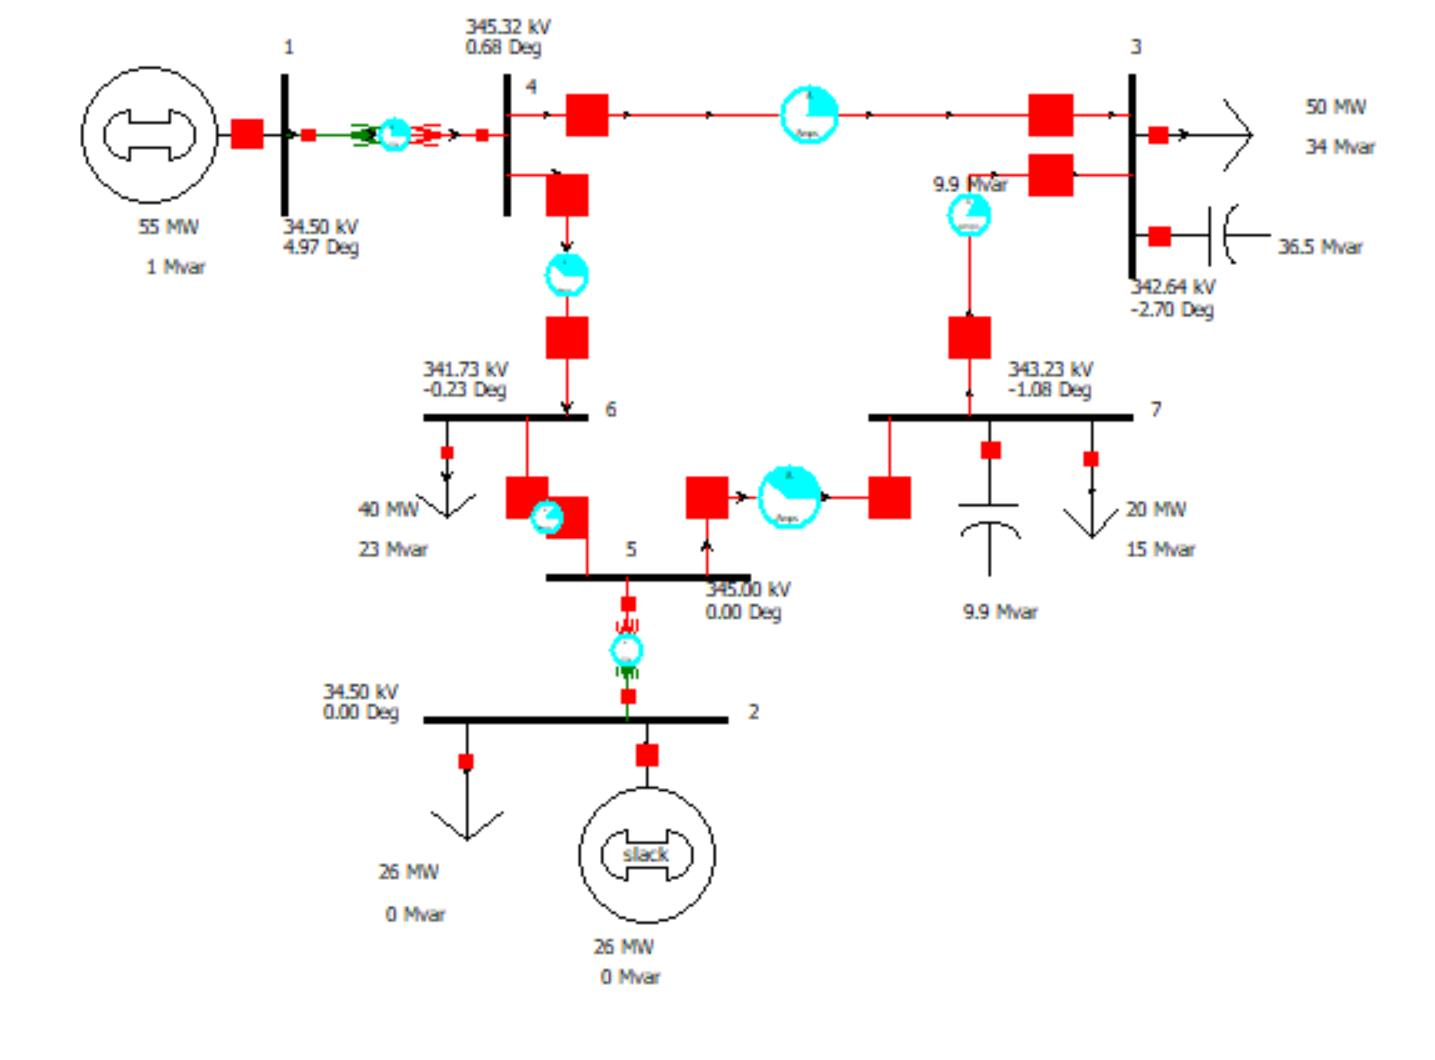
\includegraphics[width=\linewidth,height=.72\textheight,keepaspectratio]{assets/037_p001_01.png}\caption{Diagram or recorded result: Gauss-Seidel iteration.}\label{fig:037_p001_010}\end{figure}
\begin{figure}[!htbp]\centering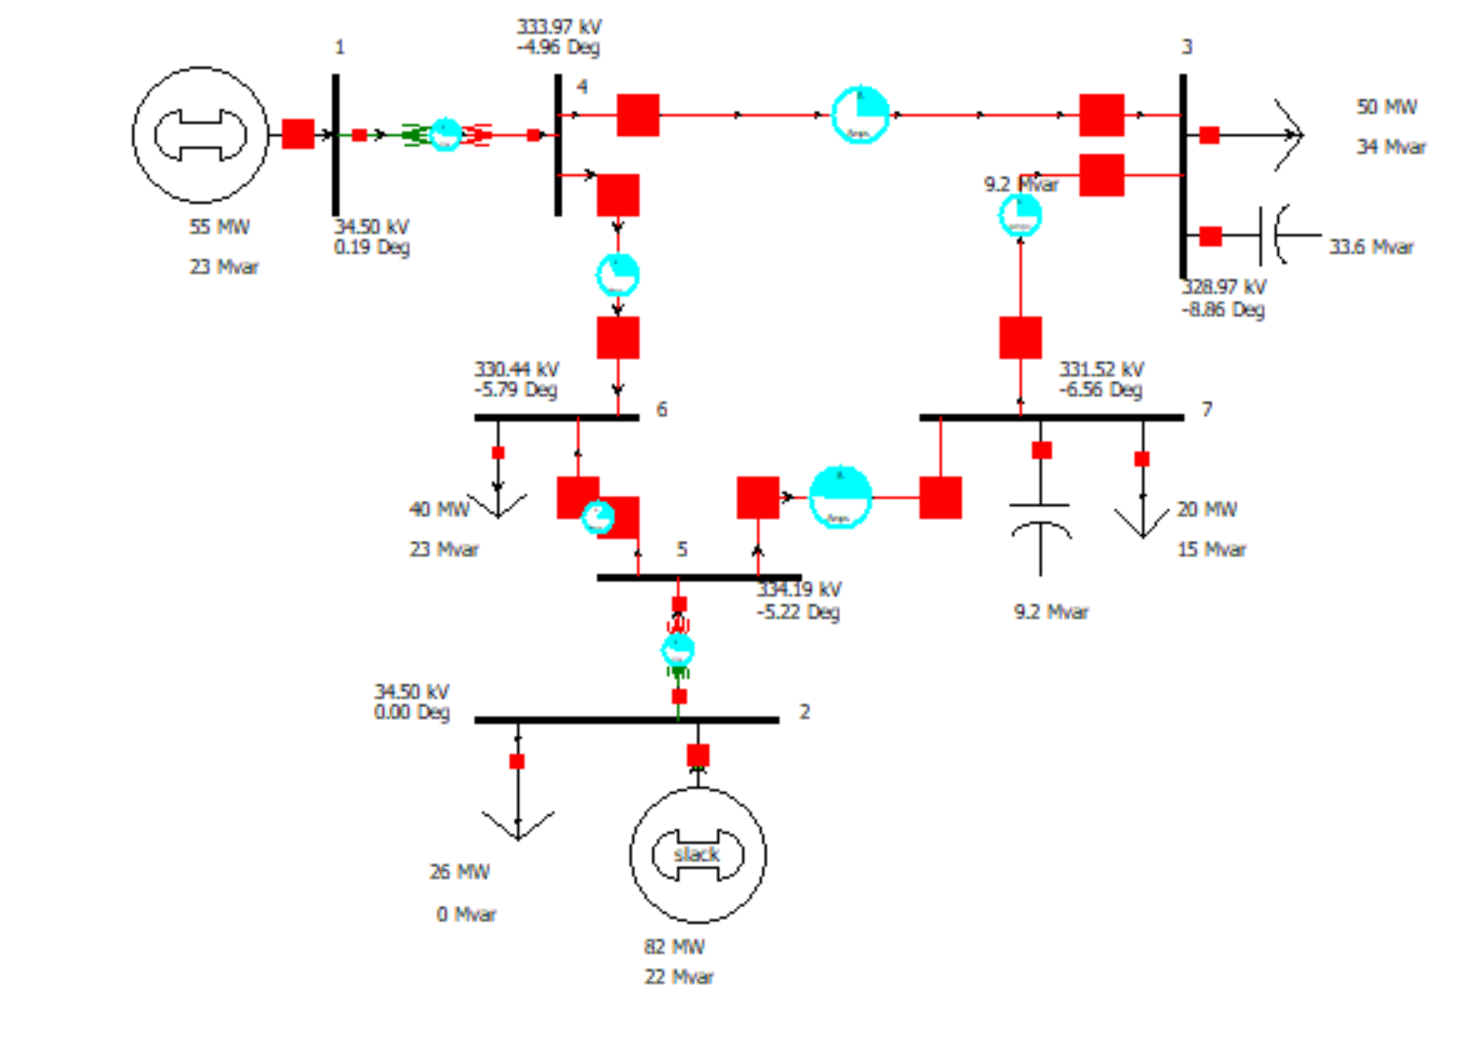
\includegraphics[width=\linewidth,height=.72\textheight,keepaspectratio]{assets/037_p002_01.png}\caption{Diagram or recorded result: Gauss-Seidel iteration.}\label{fig:037_p002_010}\end{figure}
\begin{figure}[!htbp]\centering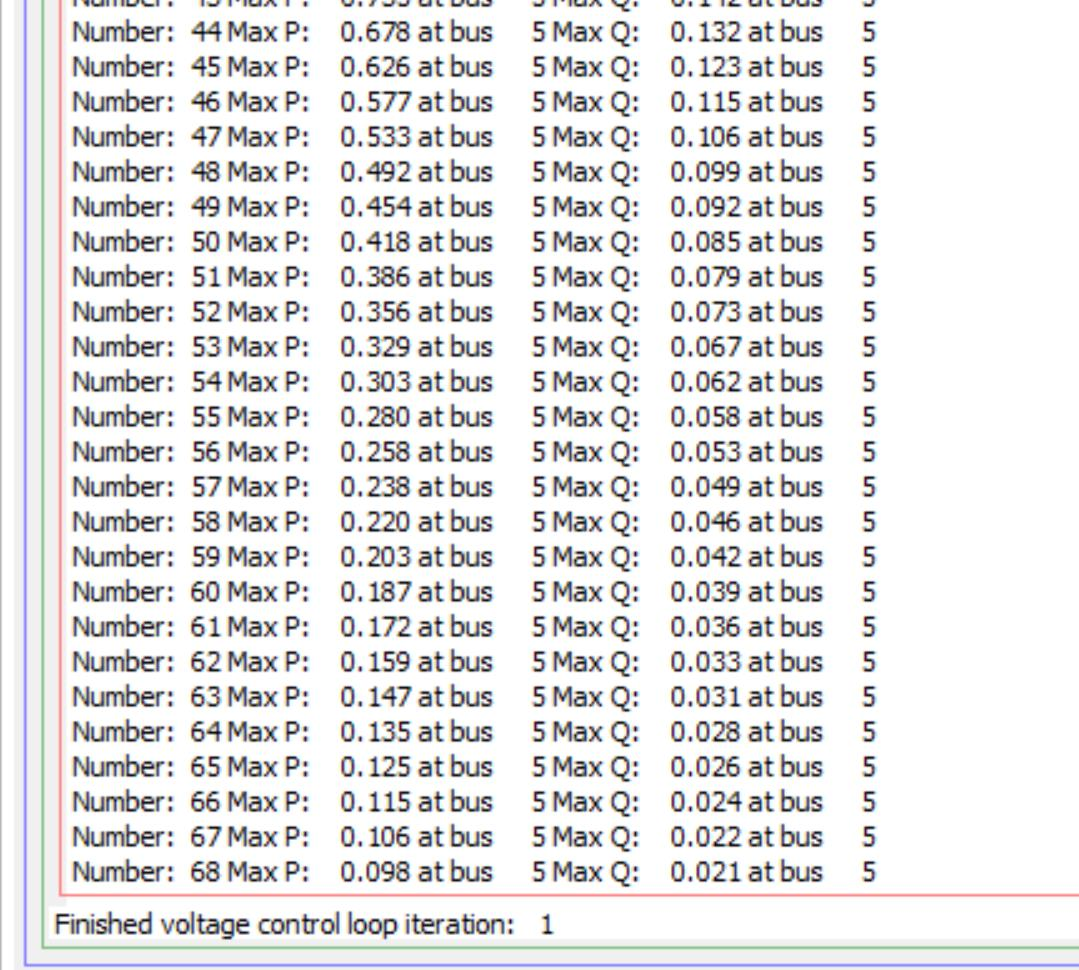
\includegraphics[width=\linewidth,height=.72\textheight,keepaspectratio]{assets/037_p003_01.png}\caption{Diagram or recorded result: Gauss-Seidel iteration.}\label{fig:037_p003_010}\end{figure}
\begin{figure}[!htbp]\centering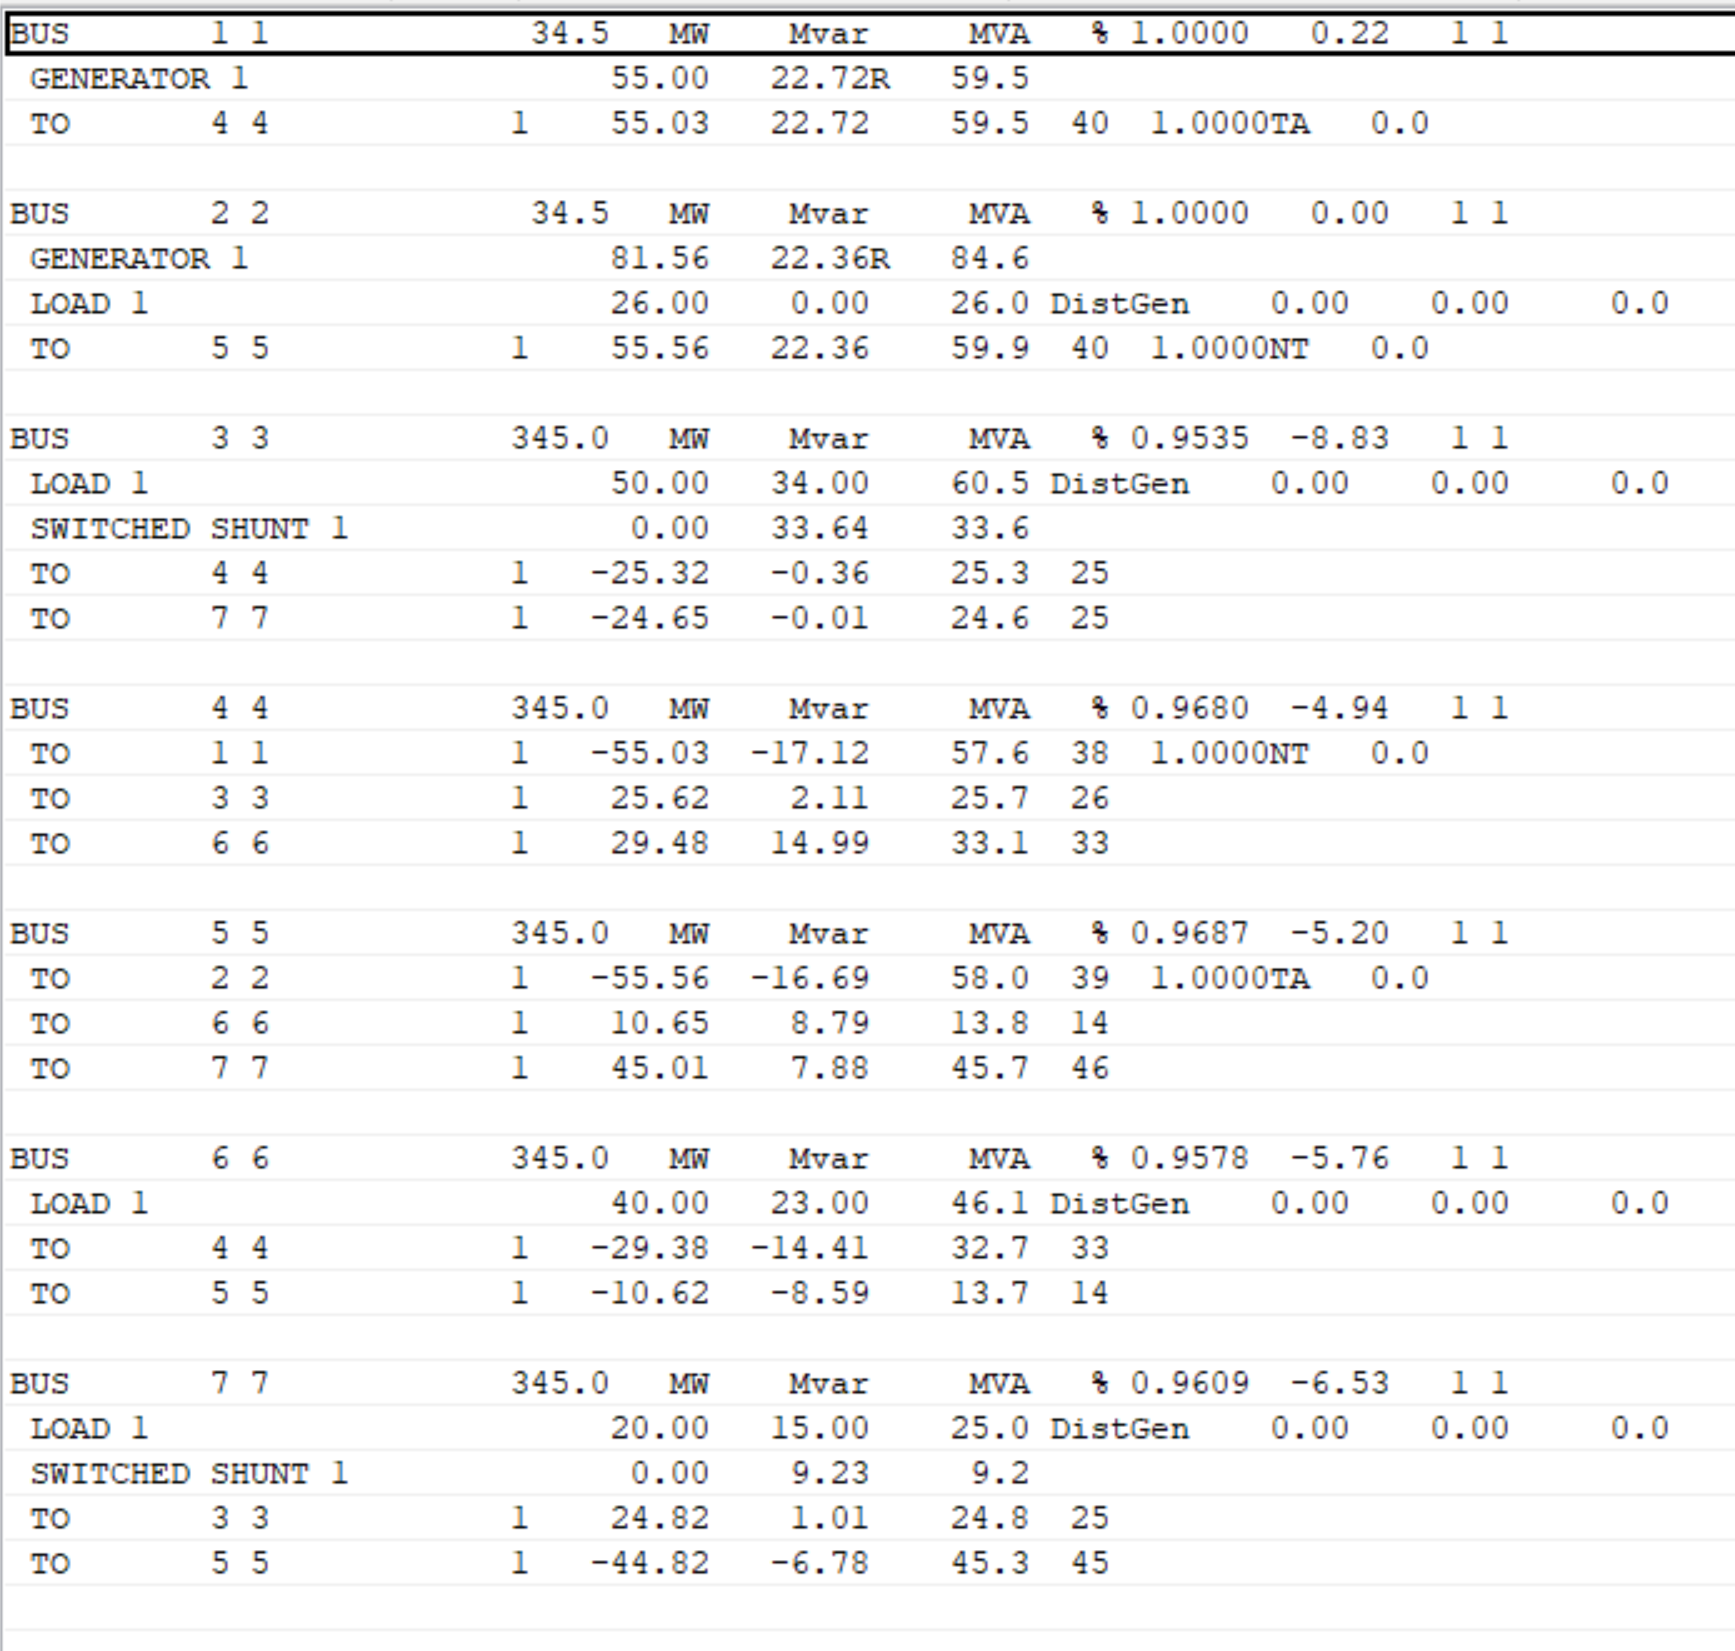
\includegraphics[width=\linewidth,height=.72\textheight,keepaspectratio]{assets/037_p004_01.png}\caption{Diagram or recorded result: Gauss-Seidel iteration.}\label{fig:037_p004_010}\end{figure}
\clearpage
\section{Newton-Raphson and Jacobian}

The corresponding Newton sequence includes one-iteration and 100-iteration settings, flow and mismatch views, and the power-flow Jacobian. Newton's local linearization can converge more rapidly near a suitable solution, but the recorded screenshots do not constitute a controlled timing benchmark. Both methods solve the same nonlinear steady-state equations;\allowbreak{} a method's convergence behavior is separate from network dynamic stability.

\begin{figure}[!htbp]\centering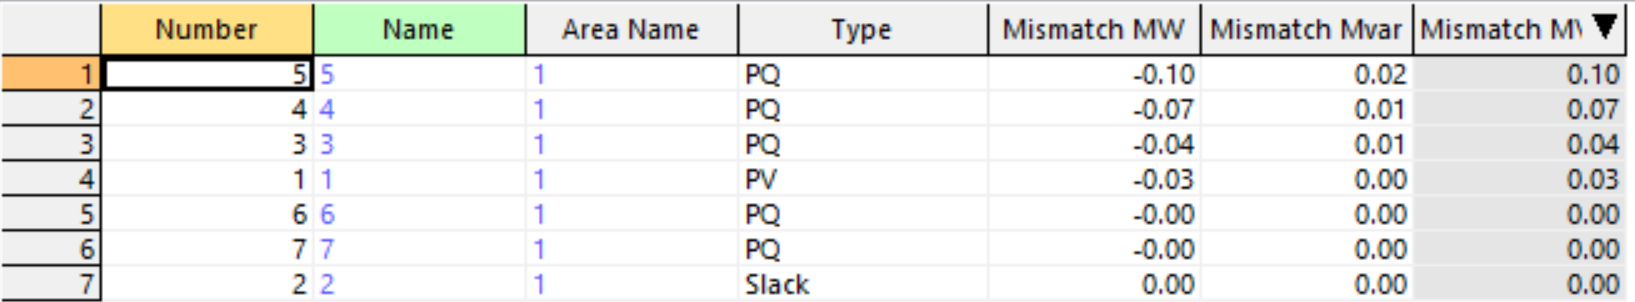
\includegraphics[width=\linewidth,height=.72\textheight,keepaspectratio]{assets/037_p005_01.png}\caption{Diagram or recorded result: Newton-Raphson and Jacobian.}\label{fig:037_p005_010}\end{figure}
\begin{figure}[!htbp]\centering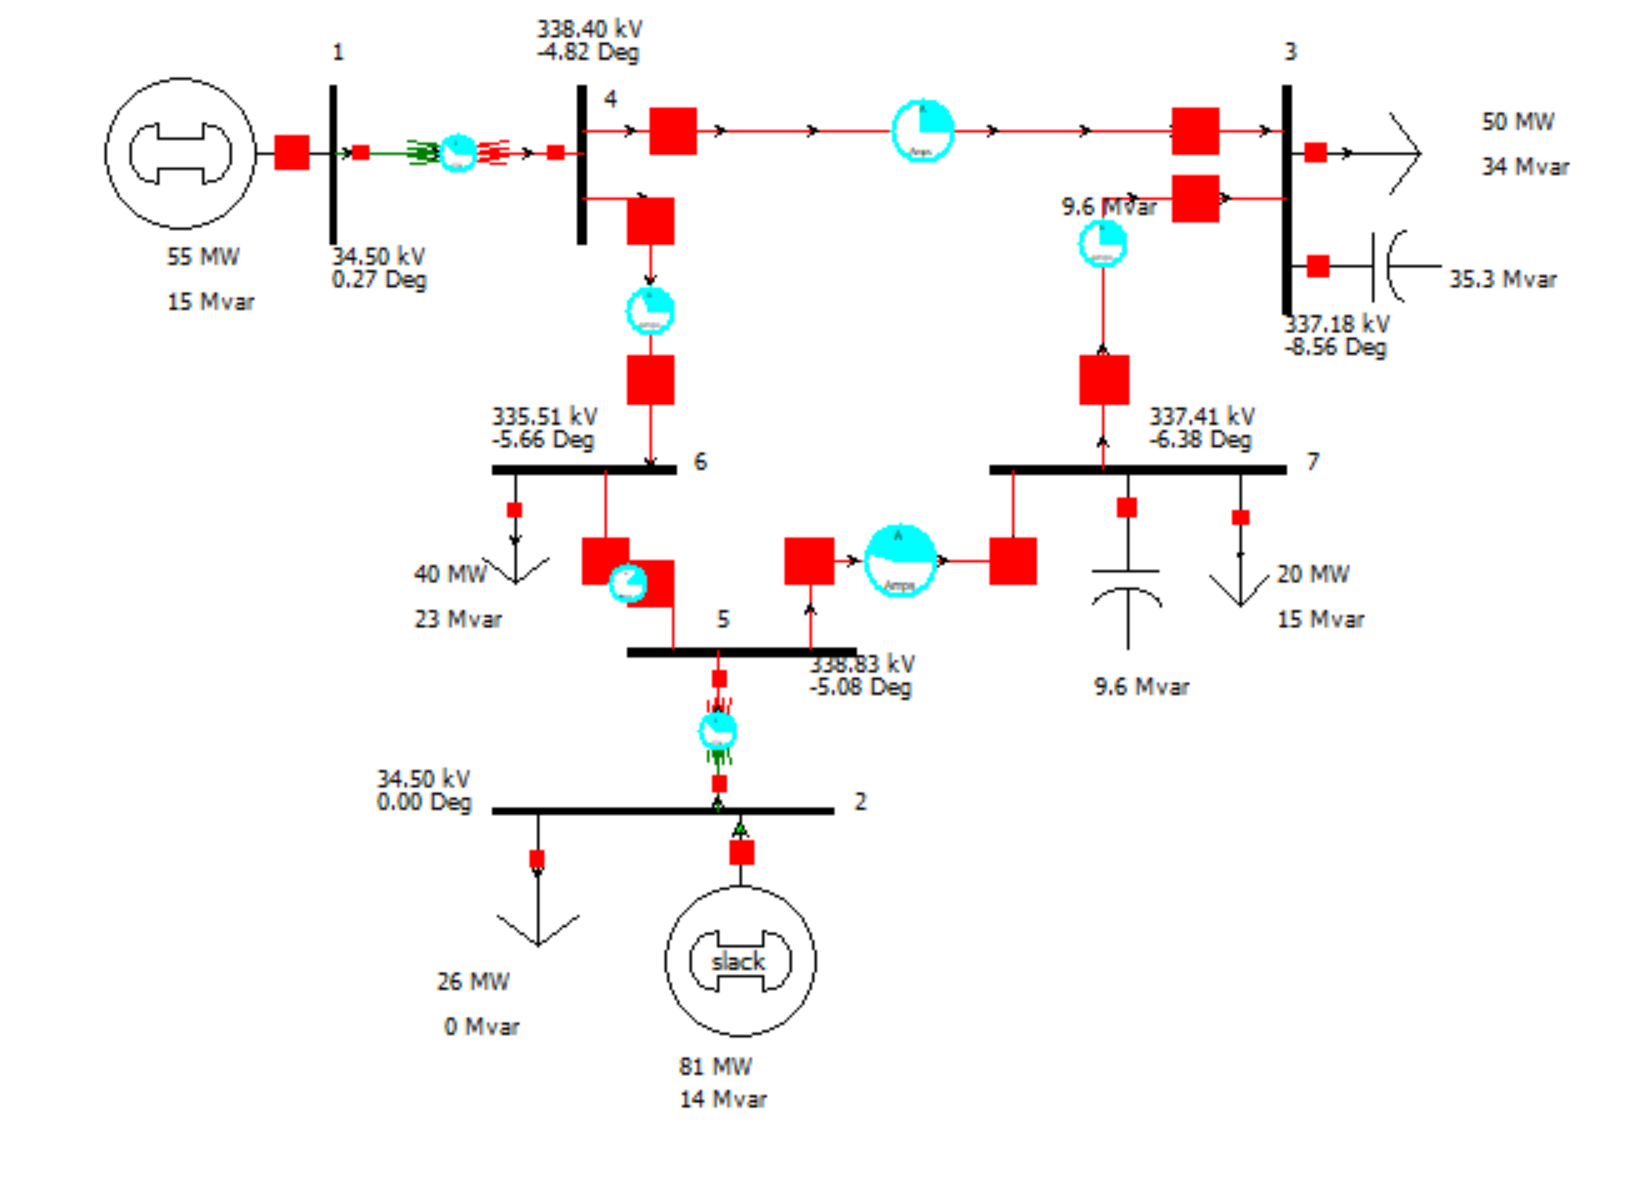
\includegraphics[width=\linewidth,height=.72\textheight,keepaspectratio]{assets/037_p005_02.png}\caption{Diagram or recorded result: Newton-Raphson and Jacobian.}\label{fig:037_p005_020}\end{figure}
\begin{figure}[!htbp]\centering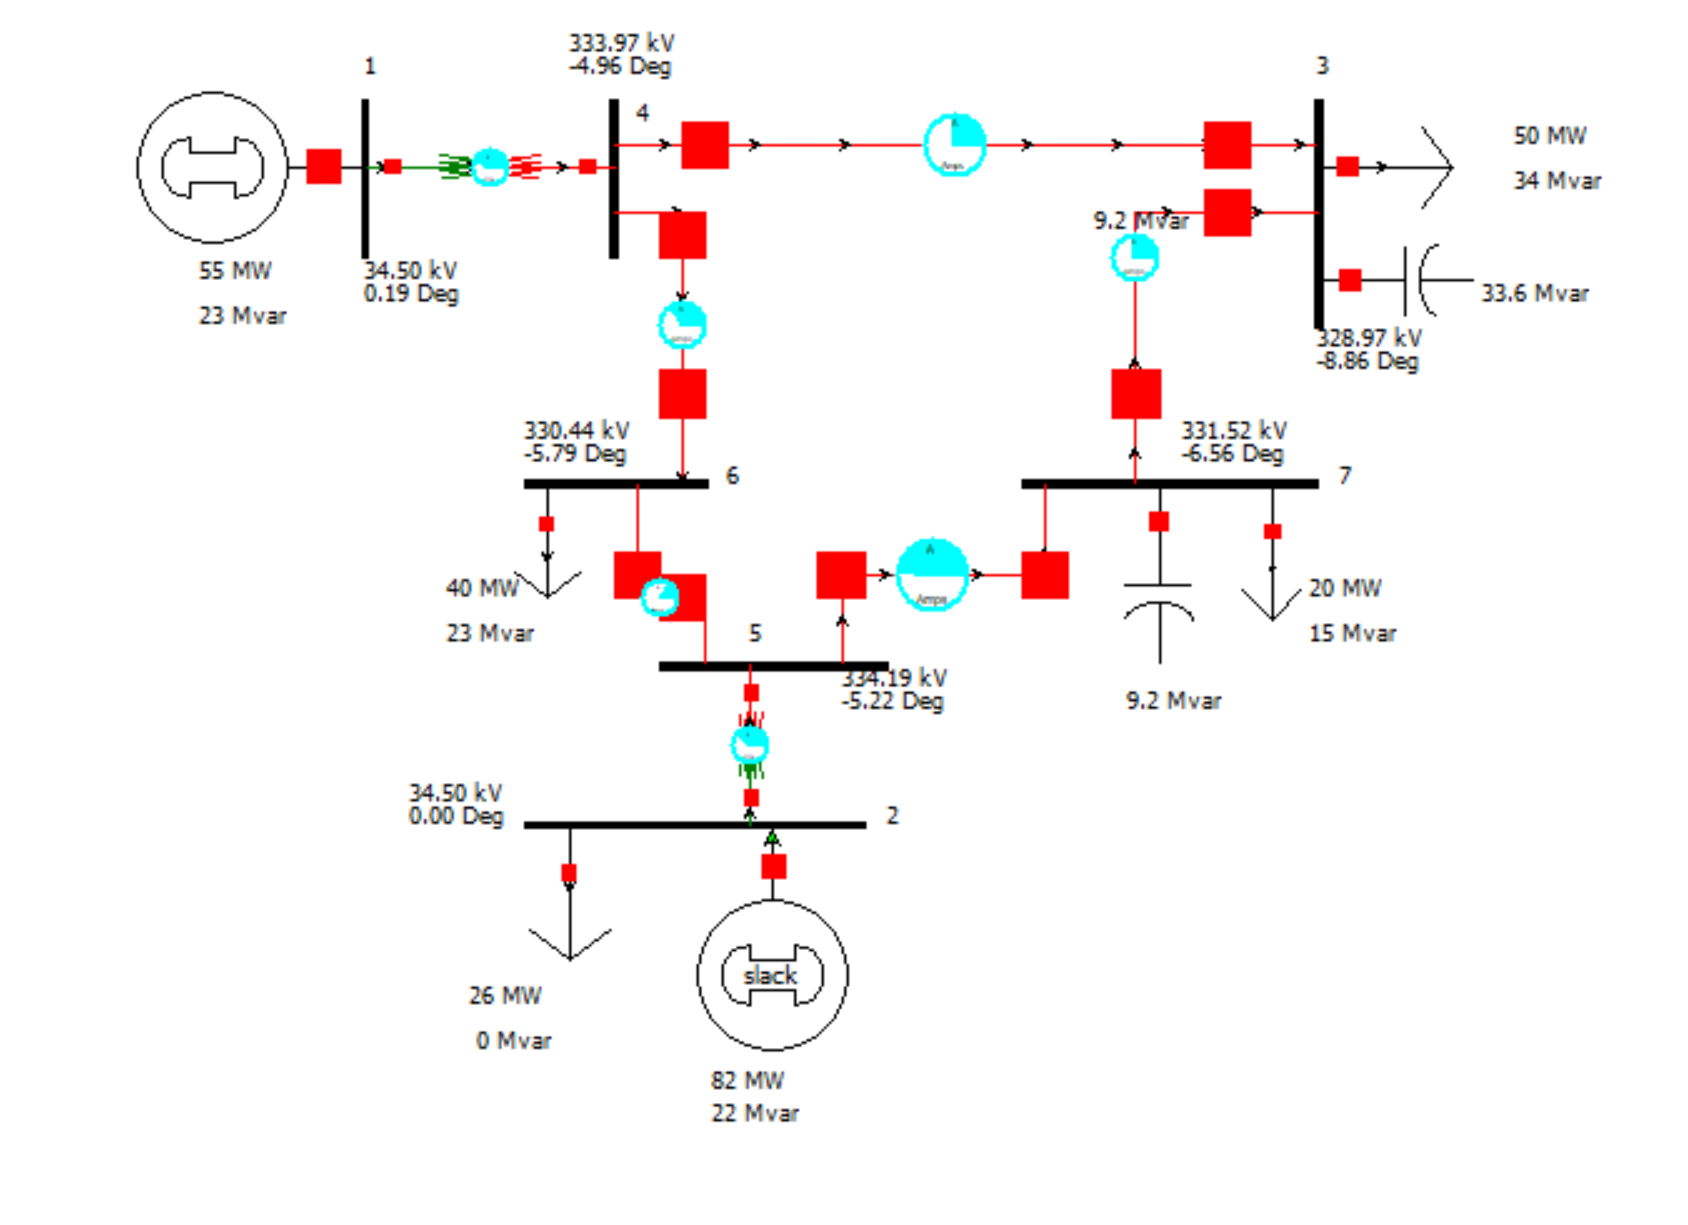
\includegraphics[width=\linewidth,height=.72\textheight,keepaspectratio]{assets/037_p006_01.png}\caption{Diagram or recorded result: Newton-Raphson and Jacobian.}\label{fig:037_p006_010}\end{figure}
\begin{figure}[!htbp]\centering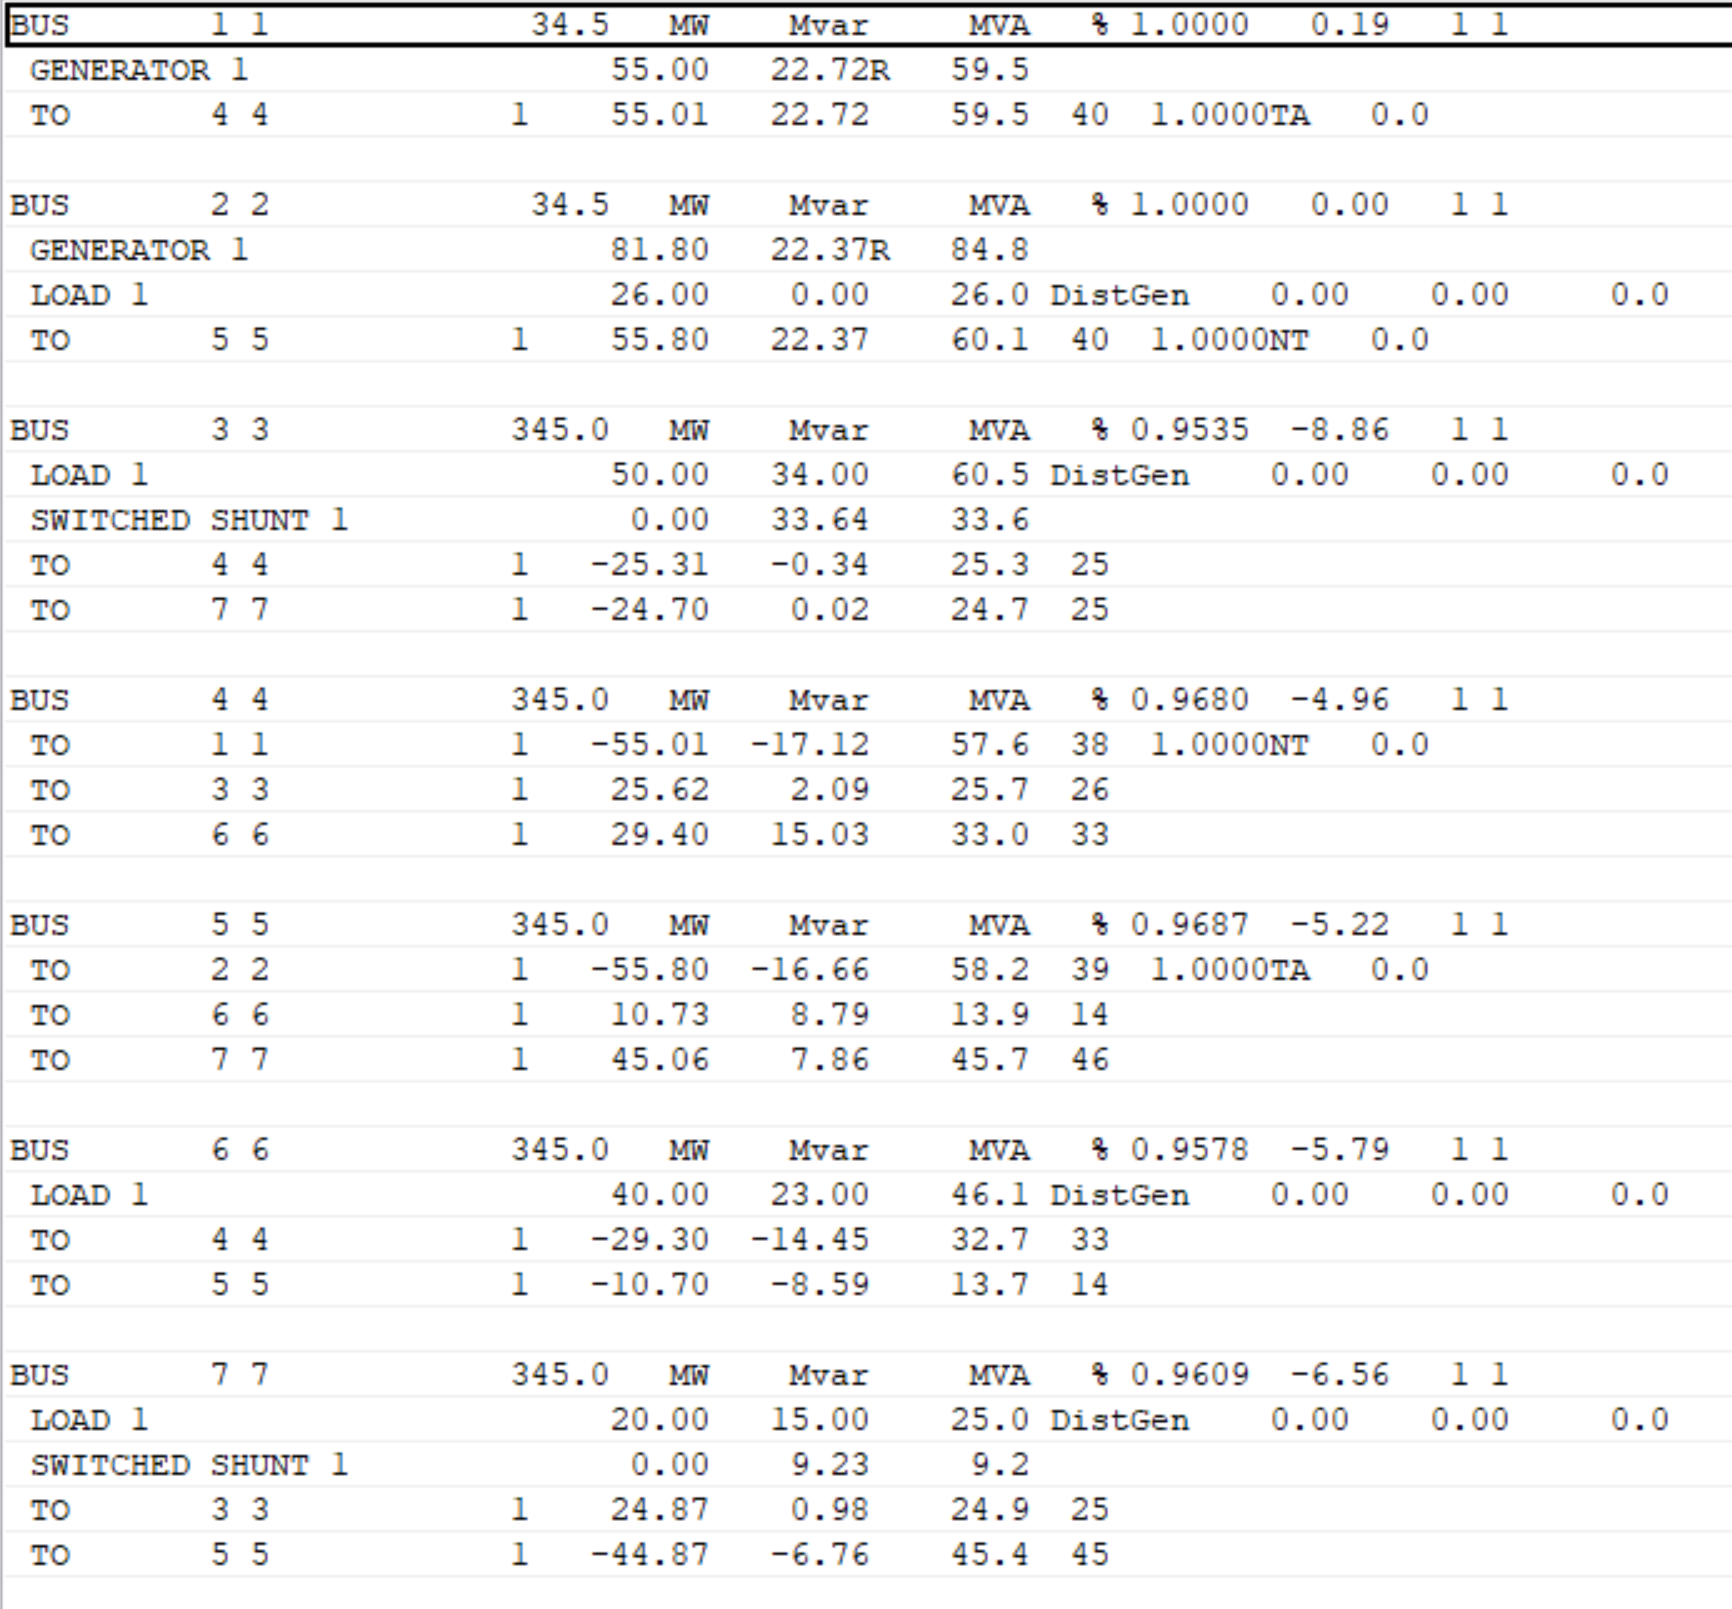
\includegraphics[width=\linewidth,height=.72\textheight,keepaspectratio]{assets/037_p007_01.png}\caption{Diagram or recorded result: Newton-Raphson and Jacobian.}\label{fig:037_p007_010}\end{figure}
\begin{figure}[!htbp]\centering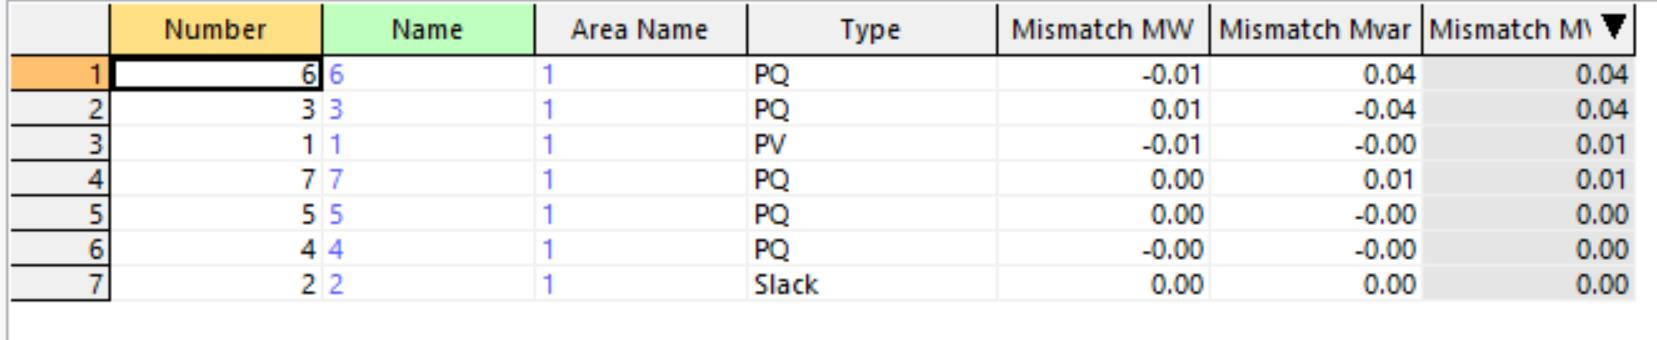
\includegraphics[width=\linewidth,height=.72\textheight,keepaspectratio]{assets/037_p007_02.png}\caption{Diagram or recorded result: Newton-Raphson and Jacobian.}\label{fig:037_p007_020}\end{figure}
\clearpage
\section{Shunt compensation and voltage limits}

With the capacitor banks connected, the report states that all bus magnitudes lie between 0.95 and 1.05 per unit. It then disconnects the bus-3 bank and displays the modified network, voltages, and losses. The report observes reduced voltages away from the controlled generator buses and higher active/\allowbreak{}reactive loss entries. Removing local capacitive support increases reactive transfer requirements. Under a constant-power load model, lower voltage can increase current demand and resistive loss. At fixed real power and voltage, decreasing power factor raises current. The causal explanation must use the actual load model. Capacitor support can reduce line current and losses and support voltage, but excessive compensation can cause overvoltage. The finite case comparison does not establish equipment lifetime or a universal optimal capacitor size.

\begin{figure}[!htbp]\centering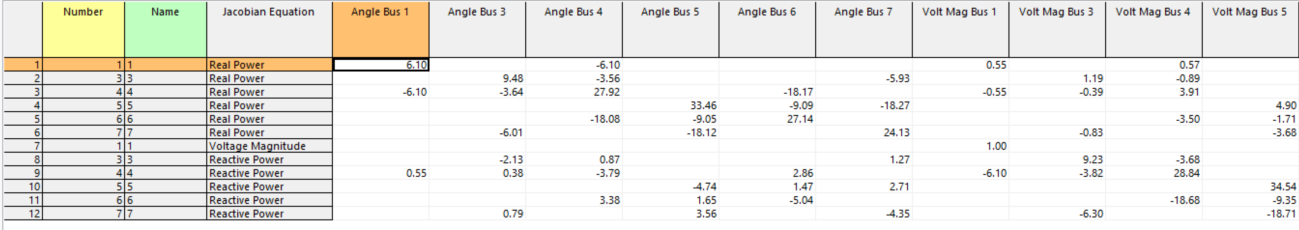
\includegraphics[width=\linewidth,height=.72\textheight,keepaspectratio]{assets/037_p008_01.png}\caption{Diagram or recorded result: Shunt compensation and voltage limits.}\label{fig:037_p008_010}\end{figure}
\begin{figure}[!htbp]\centering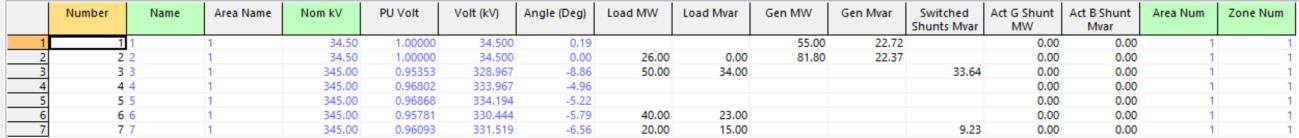
\includegraphics[width=\linewidth,height=.72\textheight,keepaspectratio]{assets/037_p008_02.png}\caption{Diagram or recorded result: Shunt compensation and voltage limits.}\label{fig:037_p008_020}\end{figure}
\begin{figure}[!htbp]\centering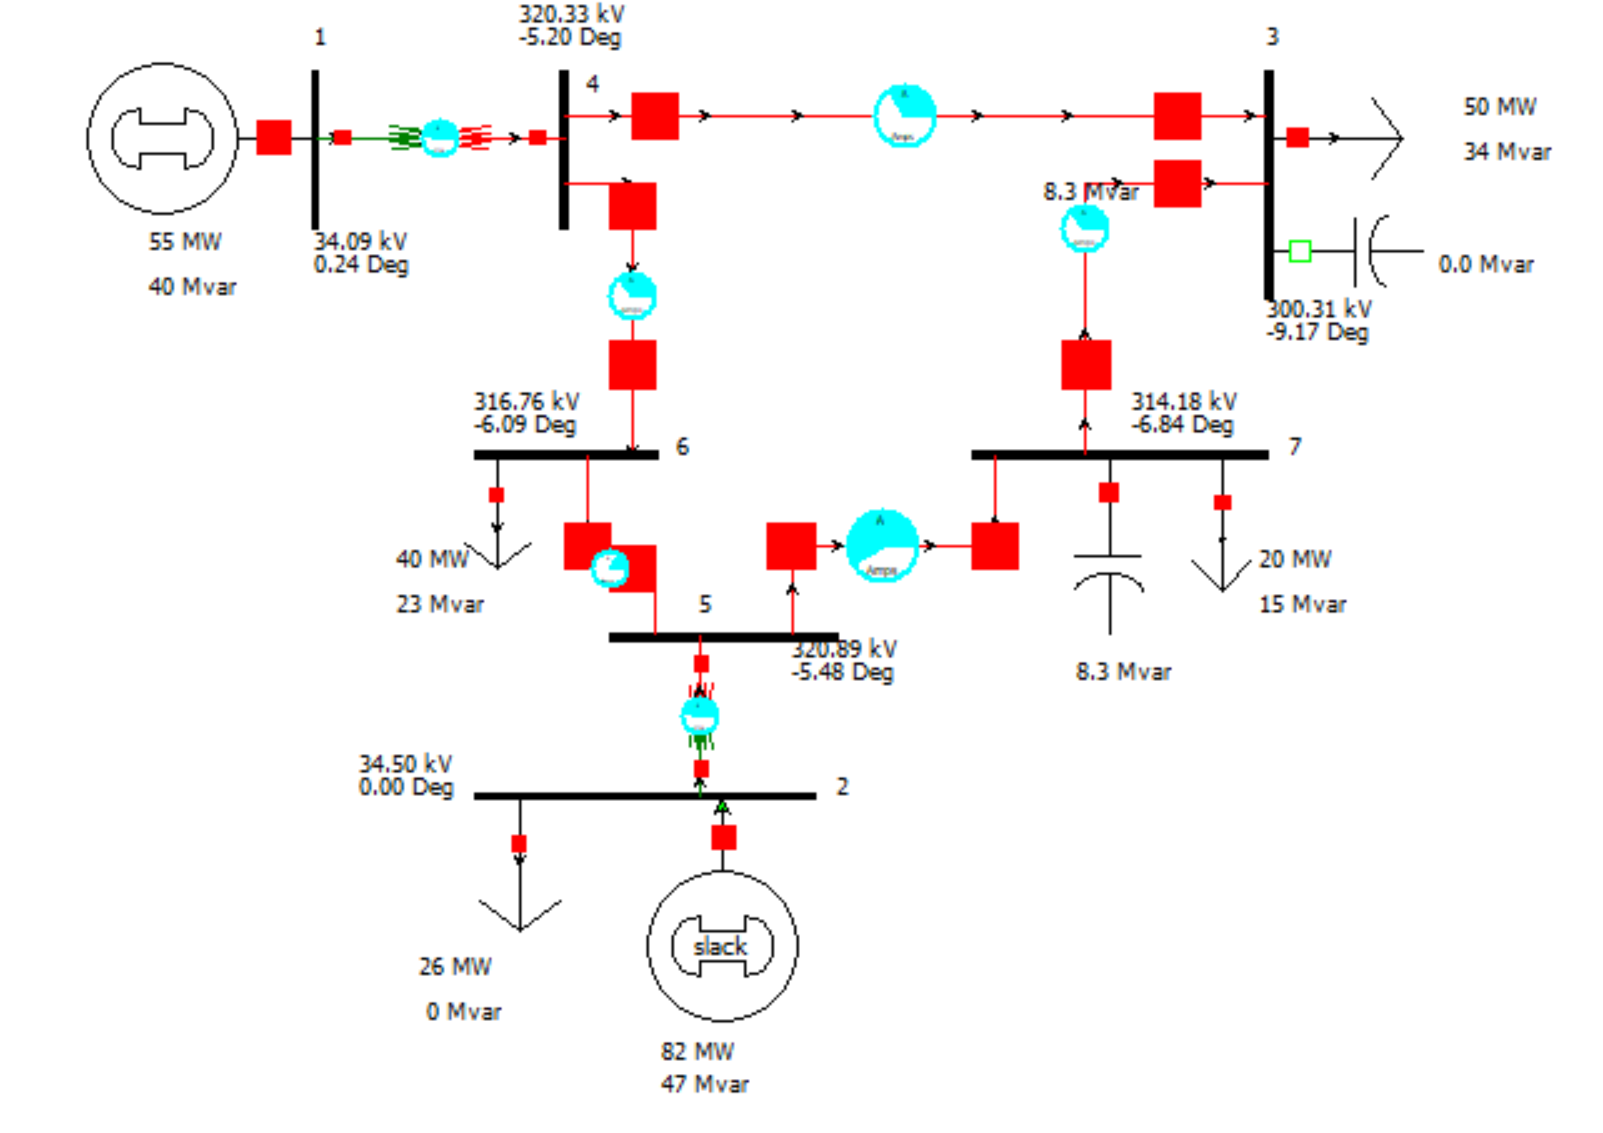
\includegraphics[width=\linewidth,height=.72\textheight,keepaspectratio]{assets/037_p009_01.png}\caption{Diagram or recorded result: Shunt compensation and voltage limits.}\label{fig:037_p009_010}\end{figure}
\clearpage
\section{Tap adjustment}

The recorded tap ratio 0.93130 brings bus 3 close to 1.0 per unit, corresponding to its 345-kV nominal level. The follow-up table is described as within all voltage limits. The controlled target is bus 3, not bus 7 or bus 1. Tap direction depends on the modeled transformer-ratio convention. The case file and tabulated bus voltages specify the observation.

\begin{figure}[!htbp]\centering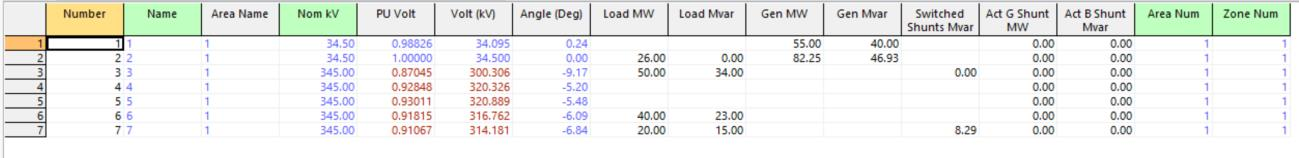
\includegraphics[width=\linewidth,height=.72\textheight,keepaspectratio]{assets/037_p010_01.png}\caption{Diagram or recorded result: Tap adjustment.}\label{fig:037_p010_010}\end{figure}
\begin{figure}[!htbp]\centering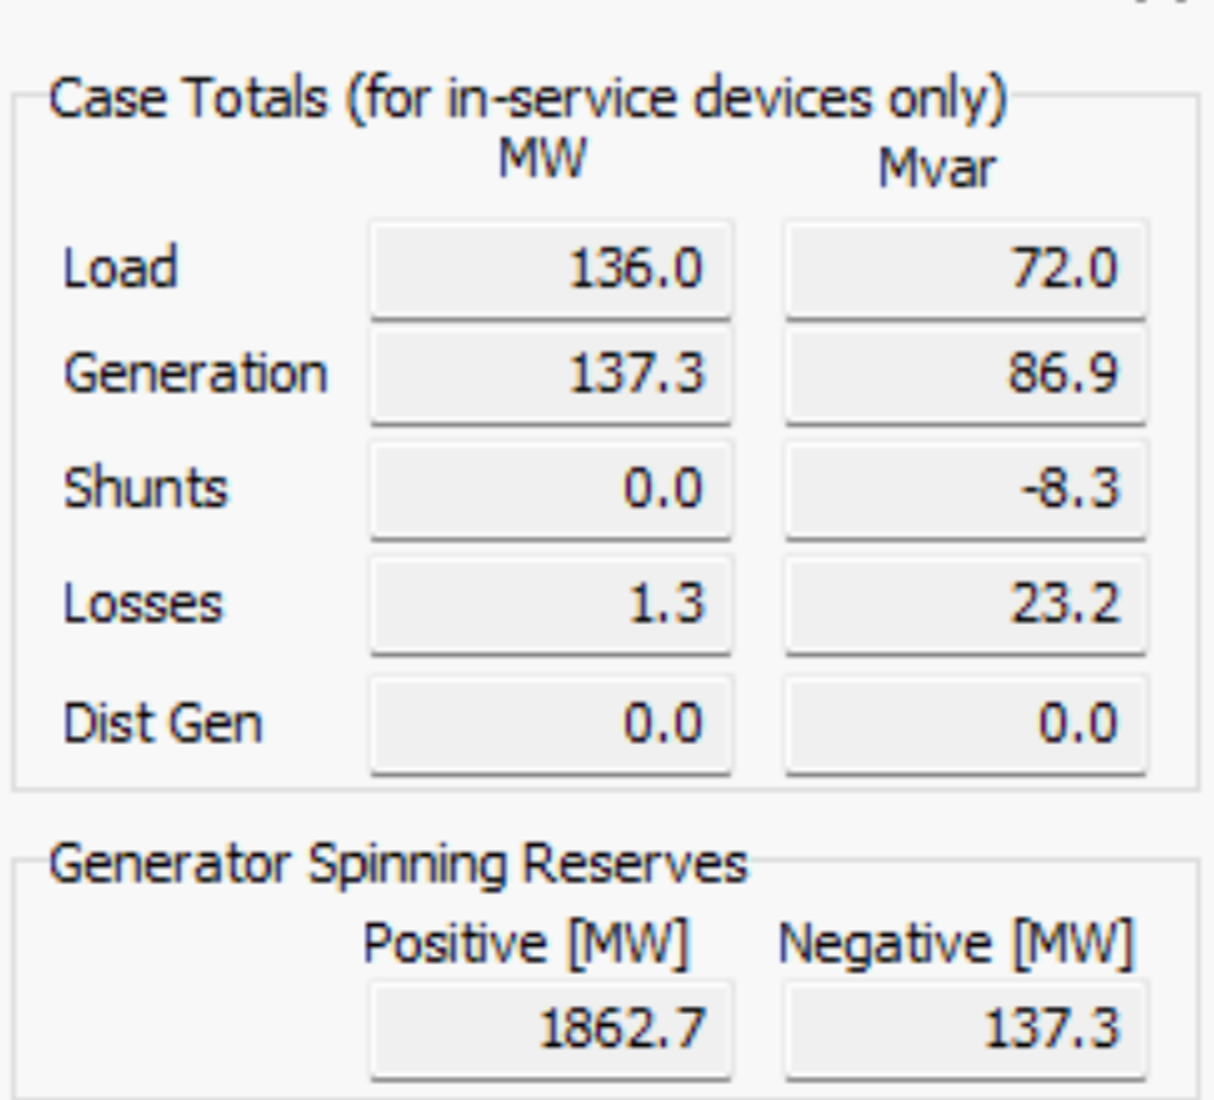
\includegraphics[width=\linewidth,height=.72\textheight,keepaspectratio]{assets/037_p011_01.png}\caption{Diagram or recorded result: Tap adjustment.}\label{fig:037_p011_010}\end{figure}
\begin{figure}[!htbp]\centering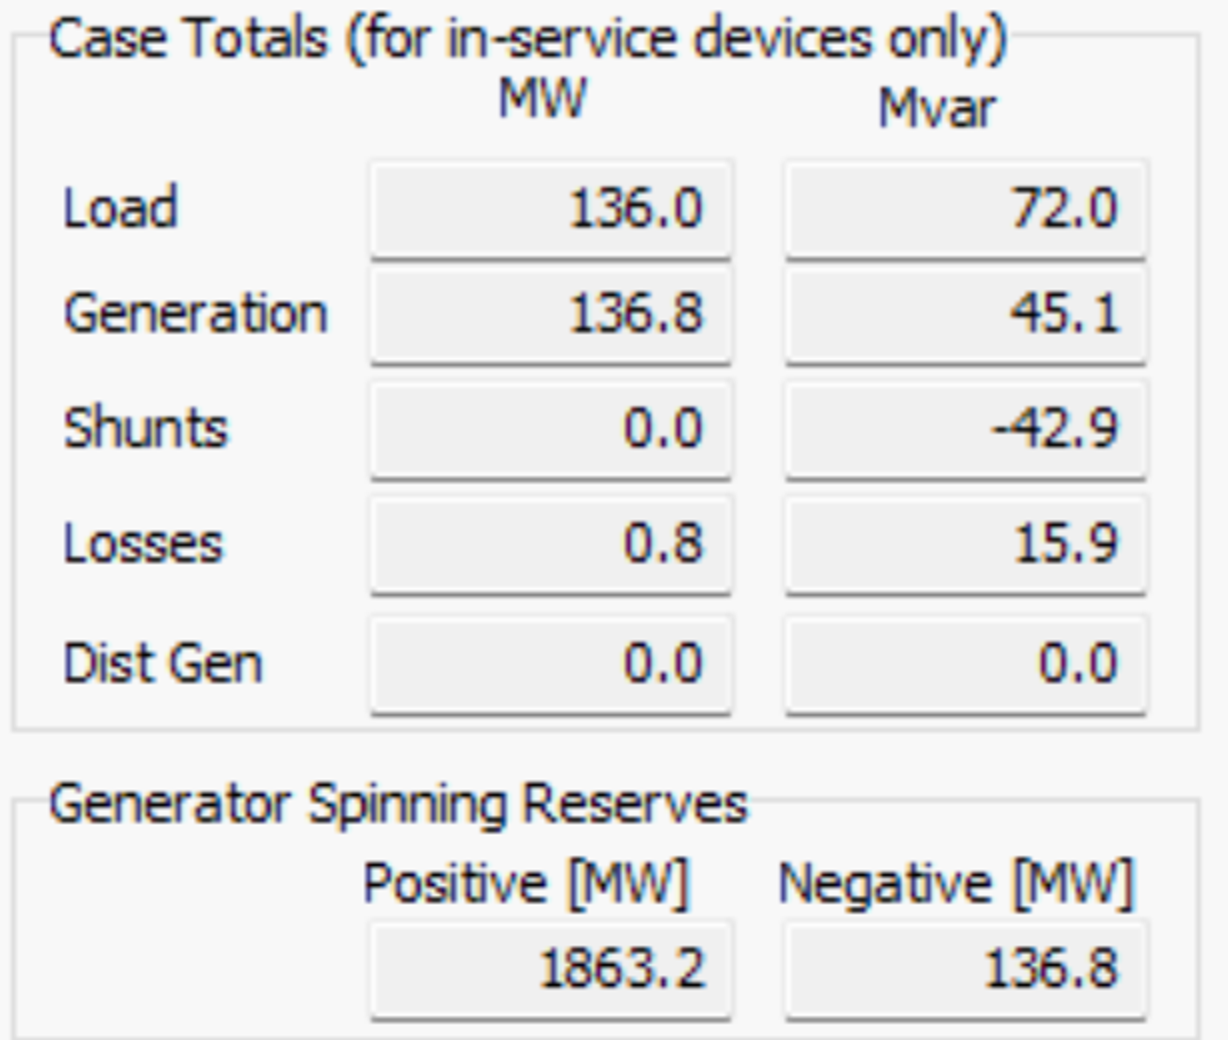
\includegraphics[width=\linewidth,height=.72\textheight,keepaspectratio]{assets/037_p012_01.png}\caption{Diagram or recorded result: Tap adjustment.}\label{fig:037_p012_010}\end{figure}
\clearpage
\section{Parallel transformers}

The report adds an identical transformer between buses 1 and 4 and records the resulting sharing. It then doubles the added transformer's reactance and displays the changed flows and bus voltages. For ideal parallel branches with compatible voltage ratios and comparable angle assumptions, lower impedance carries more current;\allowbreak{} unequal reactances prevent equal sharing. Network controls and resistances can alter the simple inverse-reactance estimate. The submitted text notes changes in reactive generation/\allowbreak{}consumption and lower voltages at buses other than the regulated generator buses in the doubled-reactance case. These are results of that edited case. The screenshots retain actual values;\allowbreak{} no new dispatch simulation is claimed here.

\begin{figure}[!htbp]\centering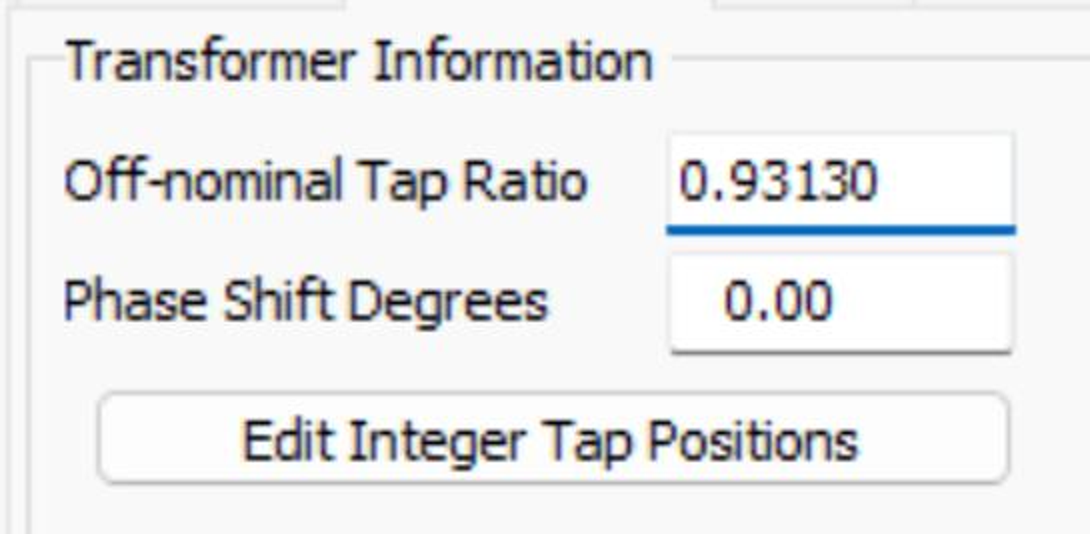
\includegraphics[width=\linewidth,height=.72\textheight,keepaspectratio]{assets/037_p013_01.png}\caption{Diagram or recorded result: Parallel transformers.}\label{fig:037_p013_010}\end{figure}
\begin{figure}[!htbp]\centering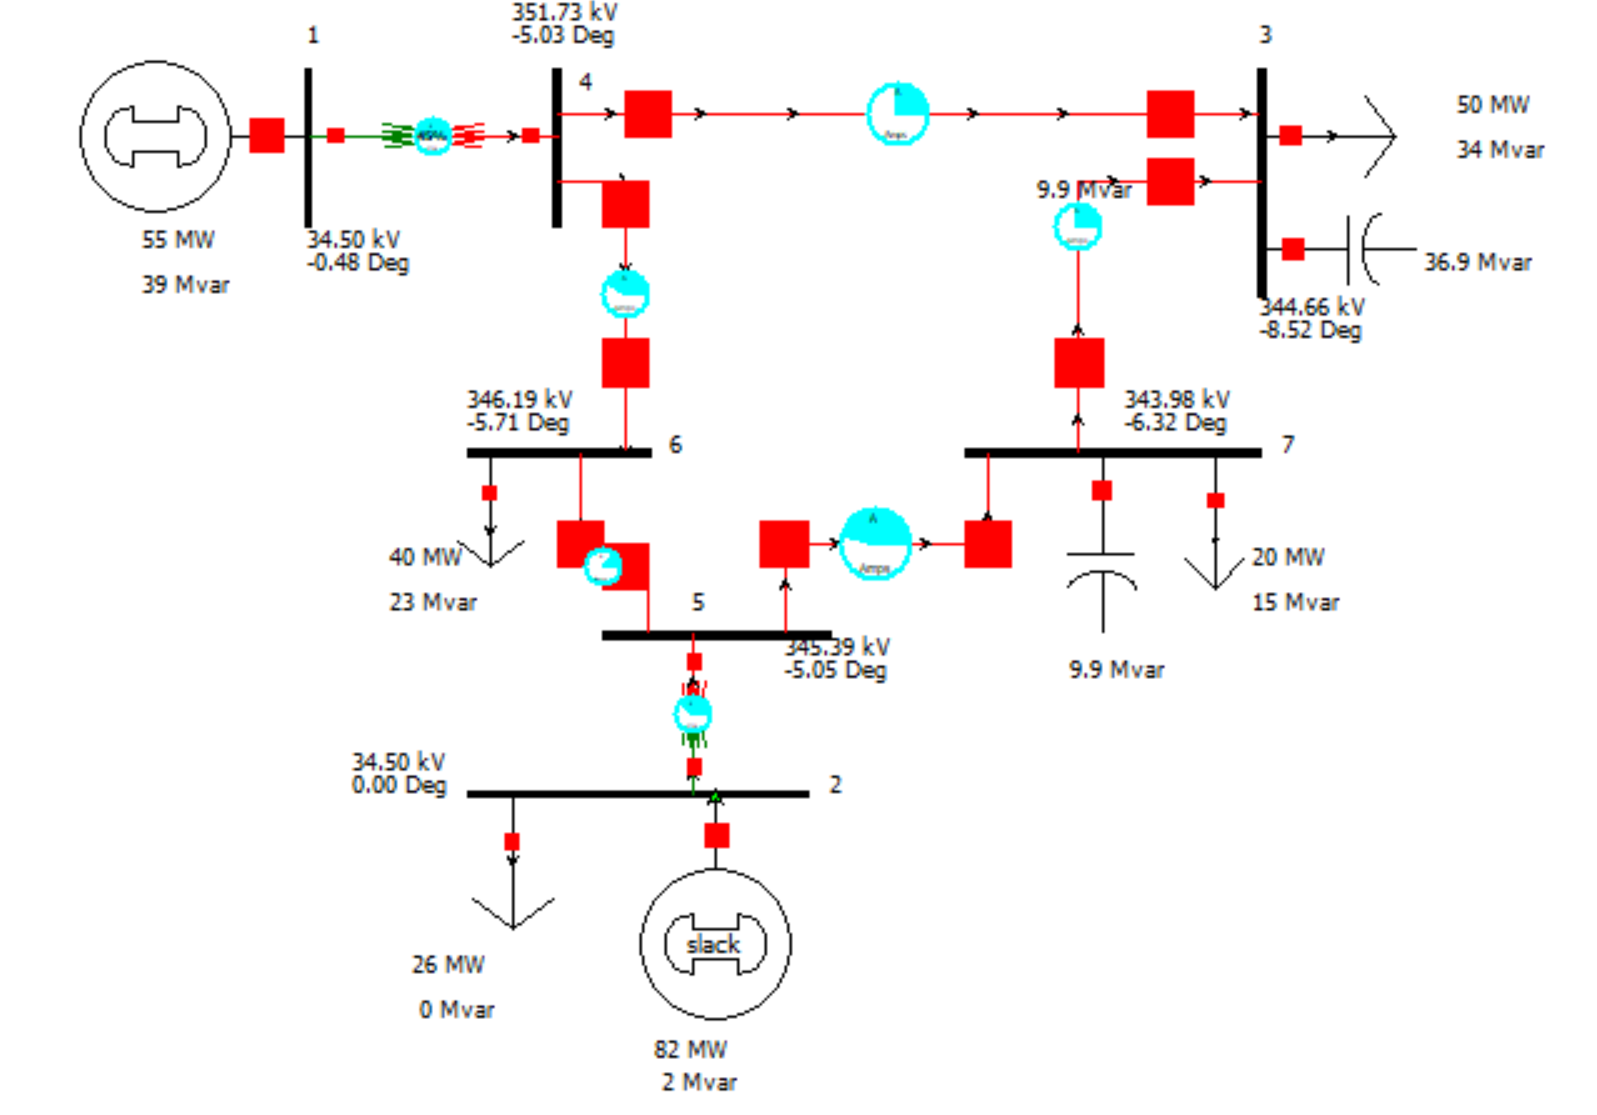
\includegraphics[width=\linewidth,height=.72\textheight,keepaspectratio]{assets/037_p014_01.png}\caption{Diagram or recorded result: Parallel transformers.}\label{fig:037_p014_010}\end{figure}
\begin{figure}[!htbp]\centering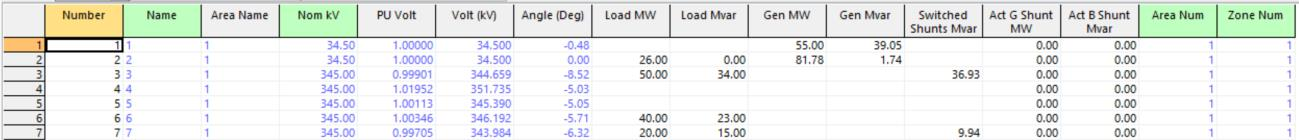
\includegraphics[width=\linewidth,height=.72\textheight,keepaspectratio]{assets/037_p015_01.png}\caption{Diagram or recorded result: Parallel transformers.}\label{fig:037_p015_010}\end{figure}
\begin{figure}[!htbp]\centering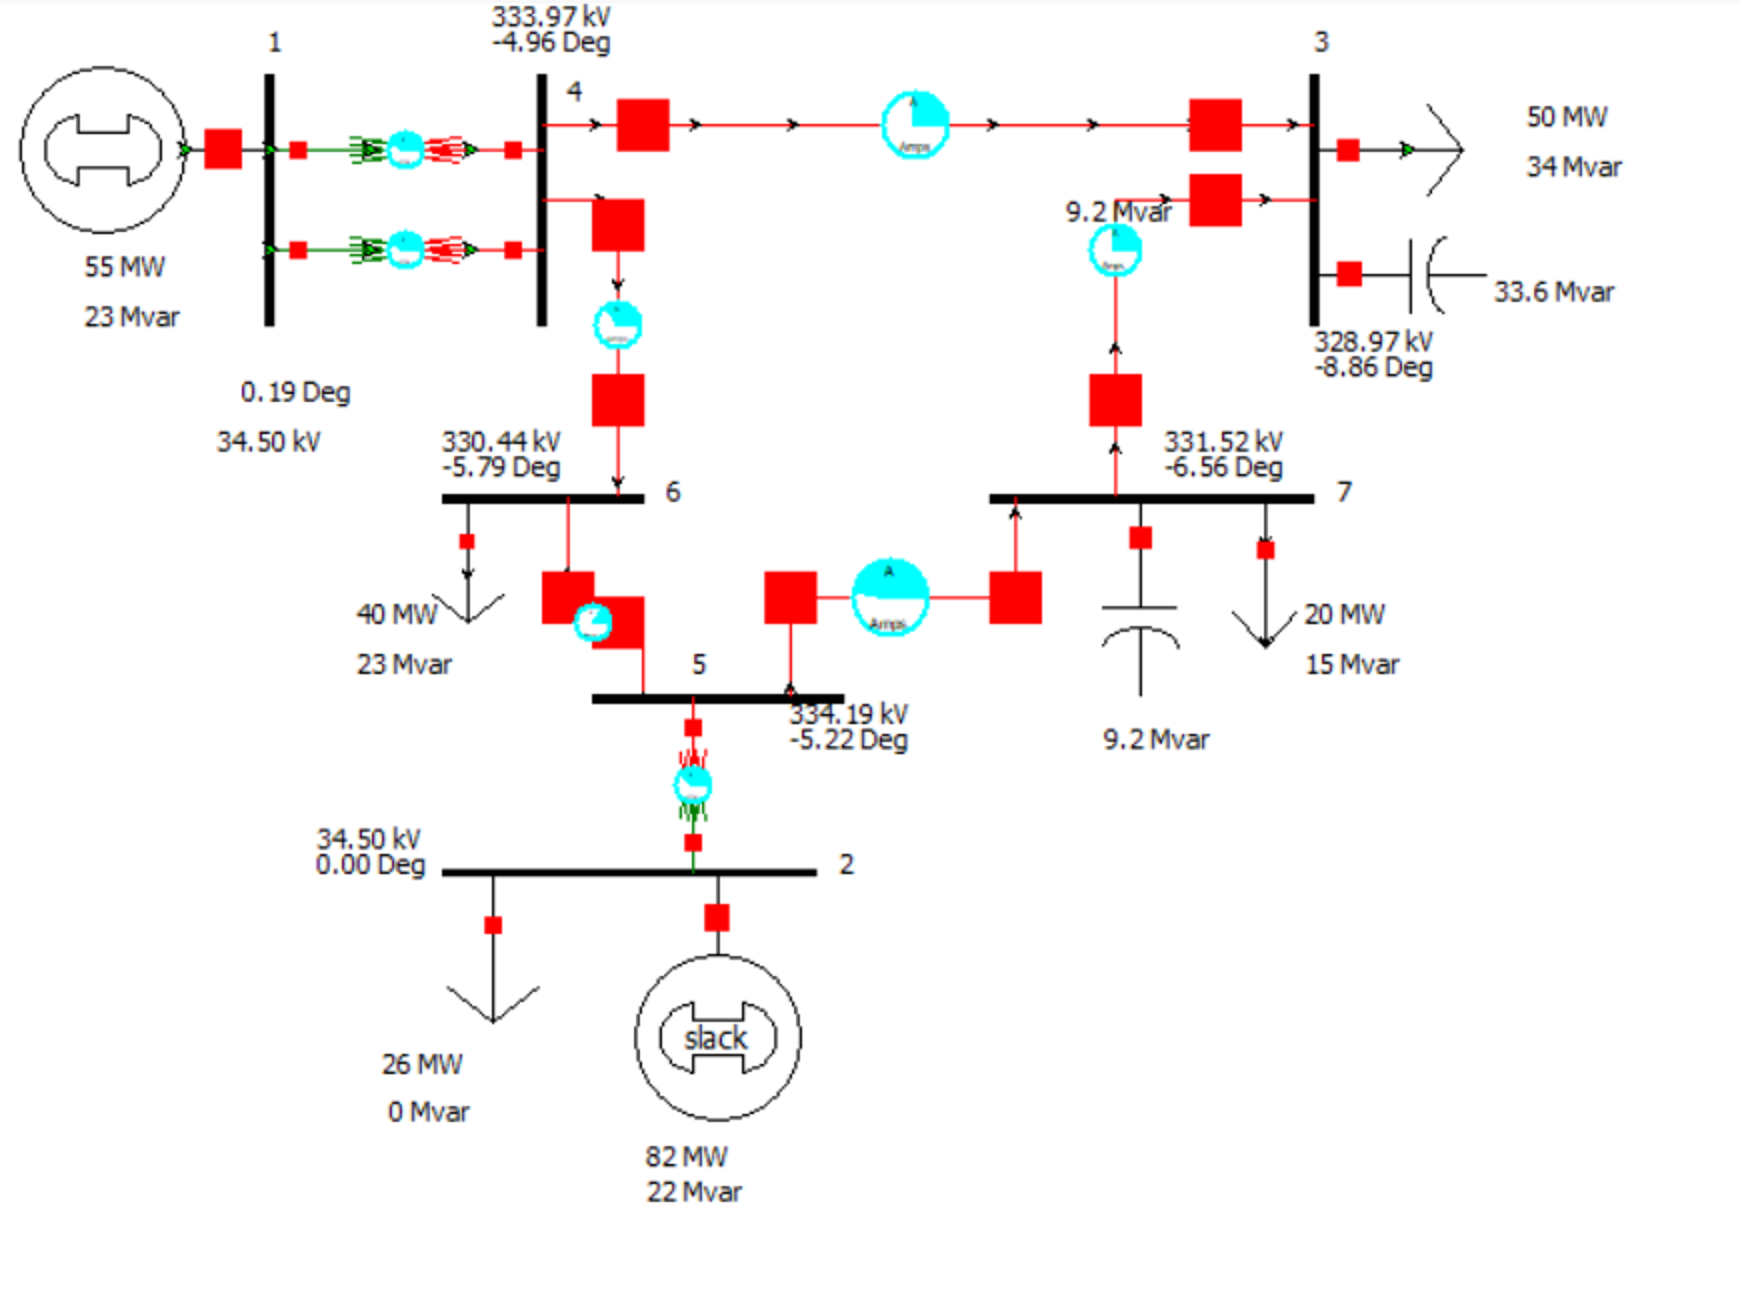
\includegraphics[width=\linewidth,height=.72\textheight,keepaspectratio]{assets/037_p015_02.png}\caption{Diagram or recorded result: Parallel transformers.}\label{fig:037_p015_020}\end{figure}
\clearpage
\section{Line outage and corrective load reduction}

After removing line 3-4, the report reduces bus-3 load to P =\allowbreak{} 40 MW and Q =\allowbreak{} 30 MVAr. Relative to the specified 50 MW/\allowbreak{}34 MVAr, this sheds 10 MW and 4 MVAr. The edited load is a demonstrated manual case adjustment, not a proved minimum shedding solution or an OPF result. A minimum would require a defined optimization objective and constraints, together with a search or optimization certificate.

\begin{figure}[!htbp]\centering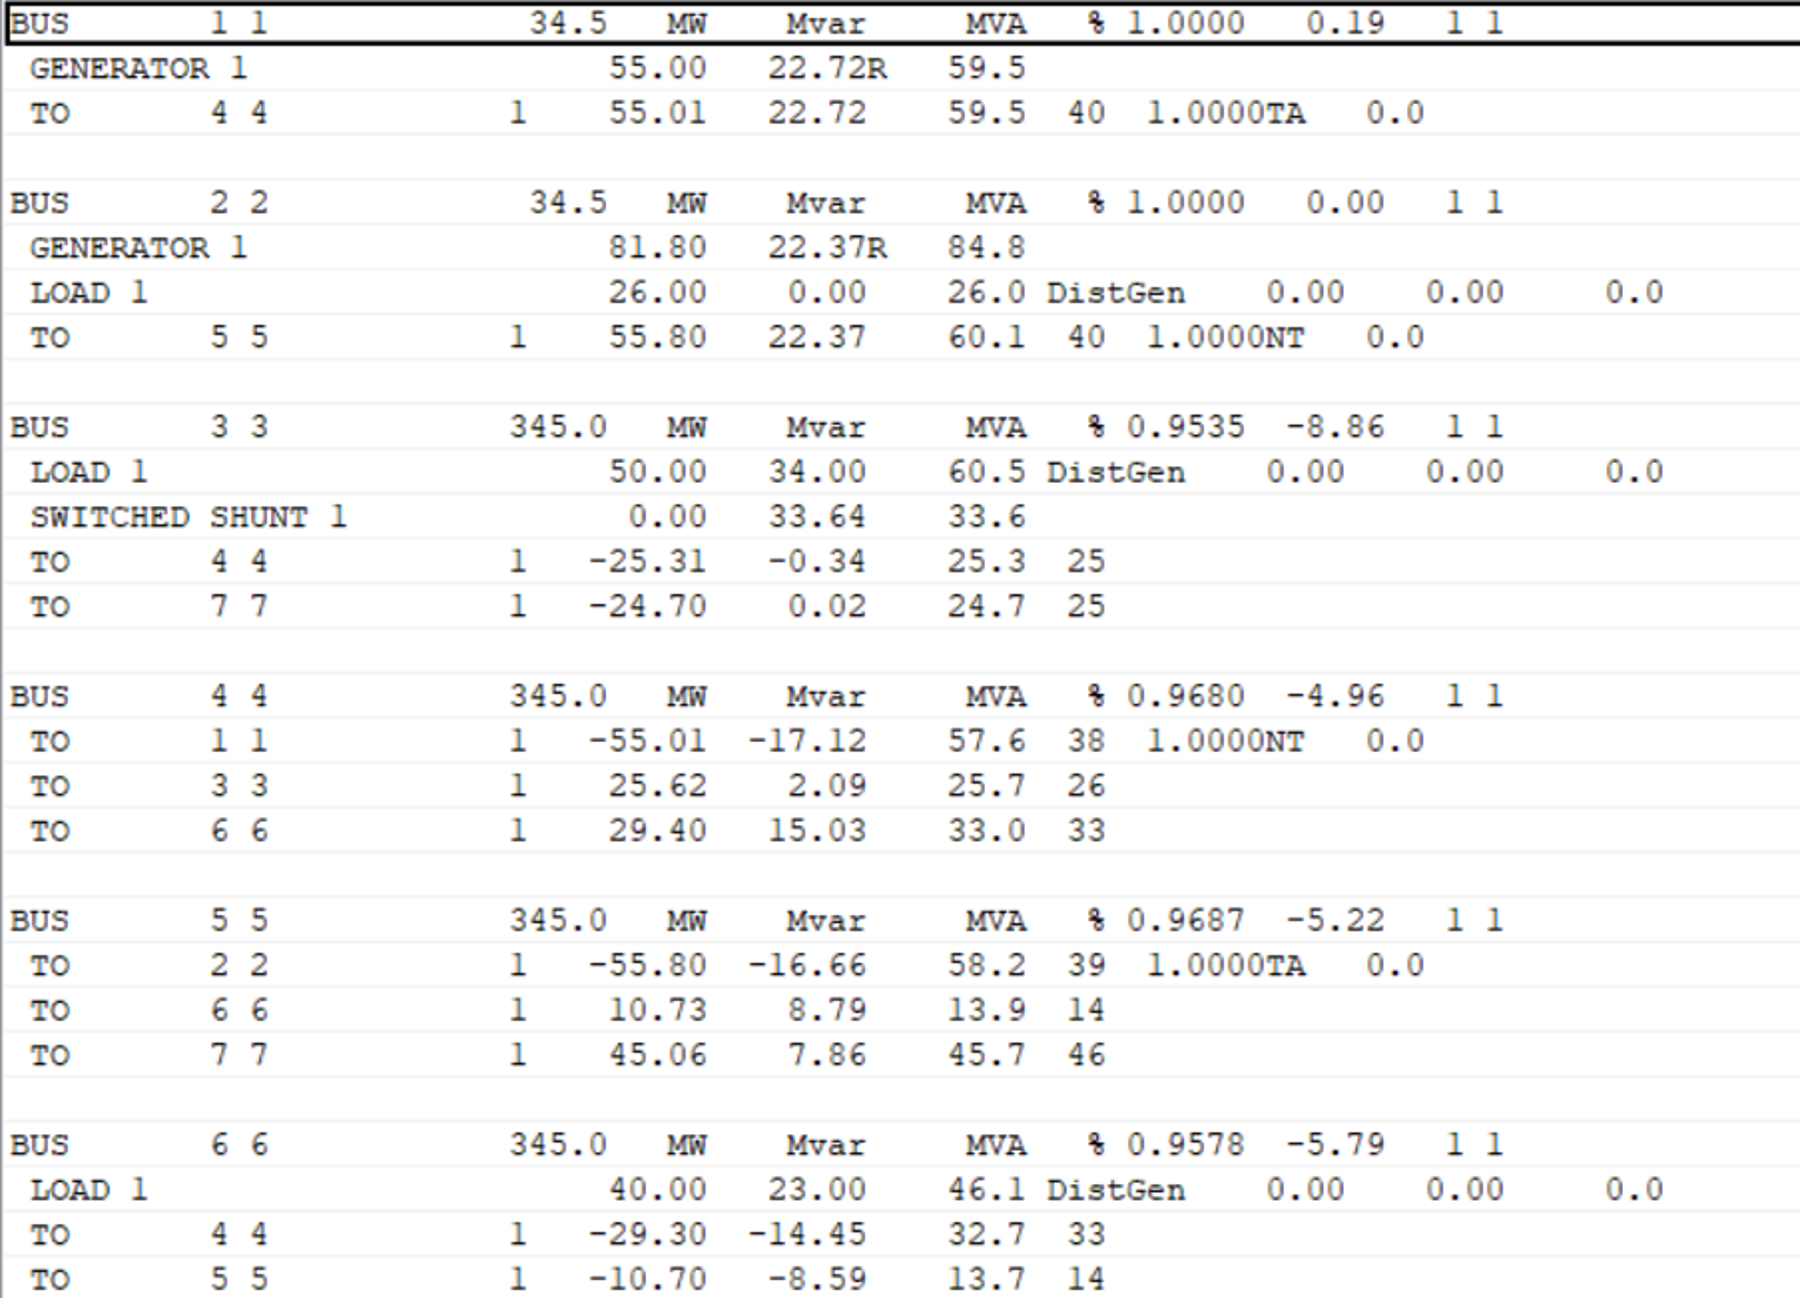
\includegraphics[width=\linewidth,height=.72\textheight,keepaspectratio]{assets/037_p016_01.png}\caption{Diagram or recorded result: Line outage and corrective load reduction.}\label{fig:037_p016_010}\end{figure}
\begin{figure}[!htbp]\centering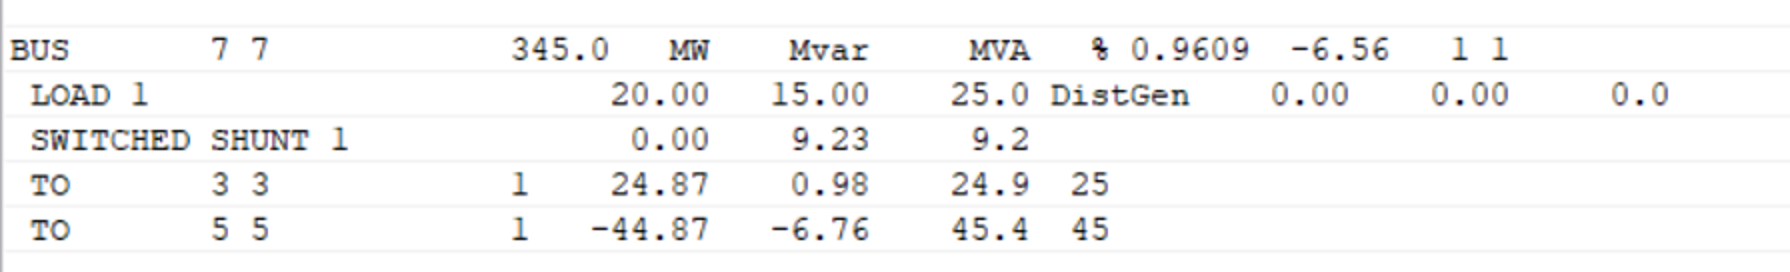
\includegraphics[width=\linewidth,height=.72\textheight,keepaspectratio]{assets/037_p016_02.png}\caption{Diagram or recorded result: Line outage and corrective load reduction.}\label{fig:037_p016_020}\end{figure}
\begin{figure}[!htbp]\centering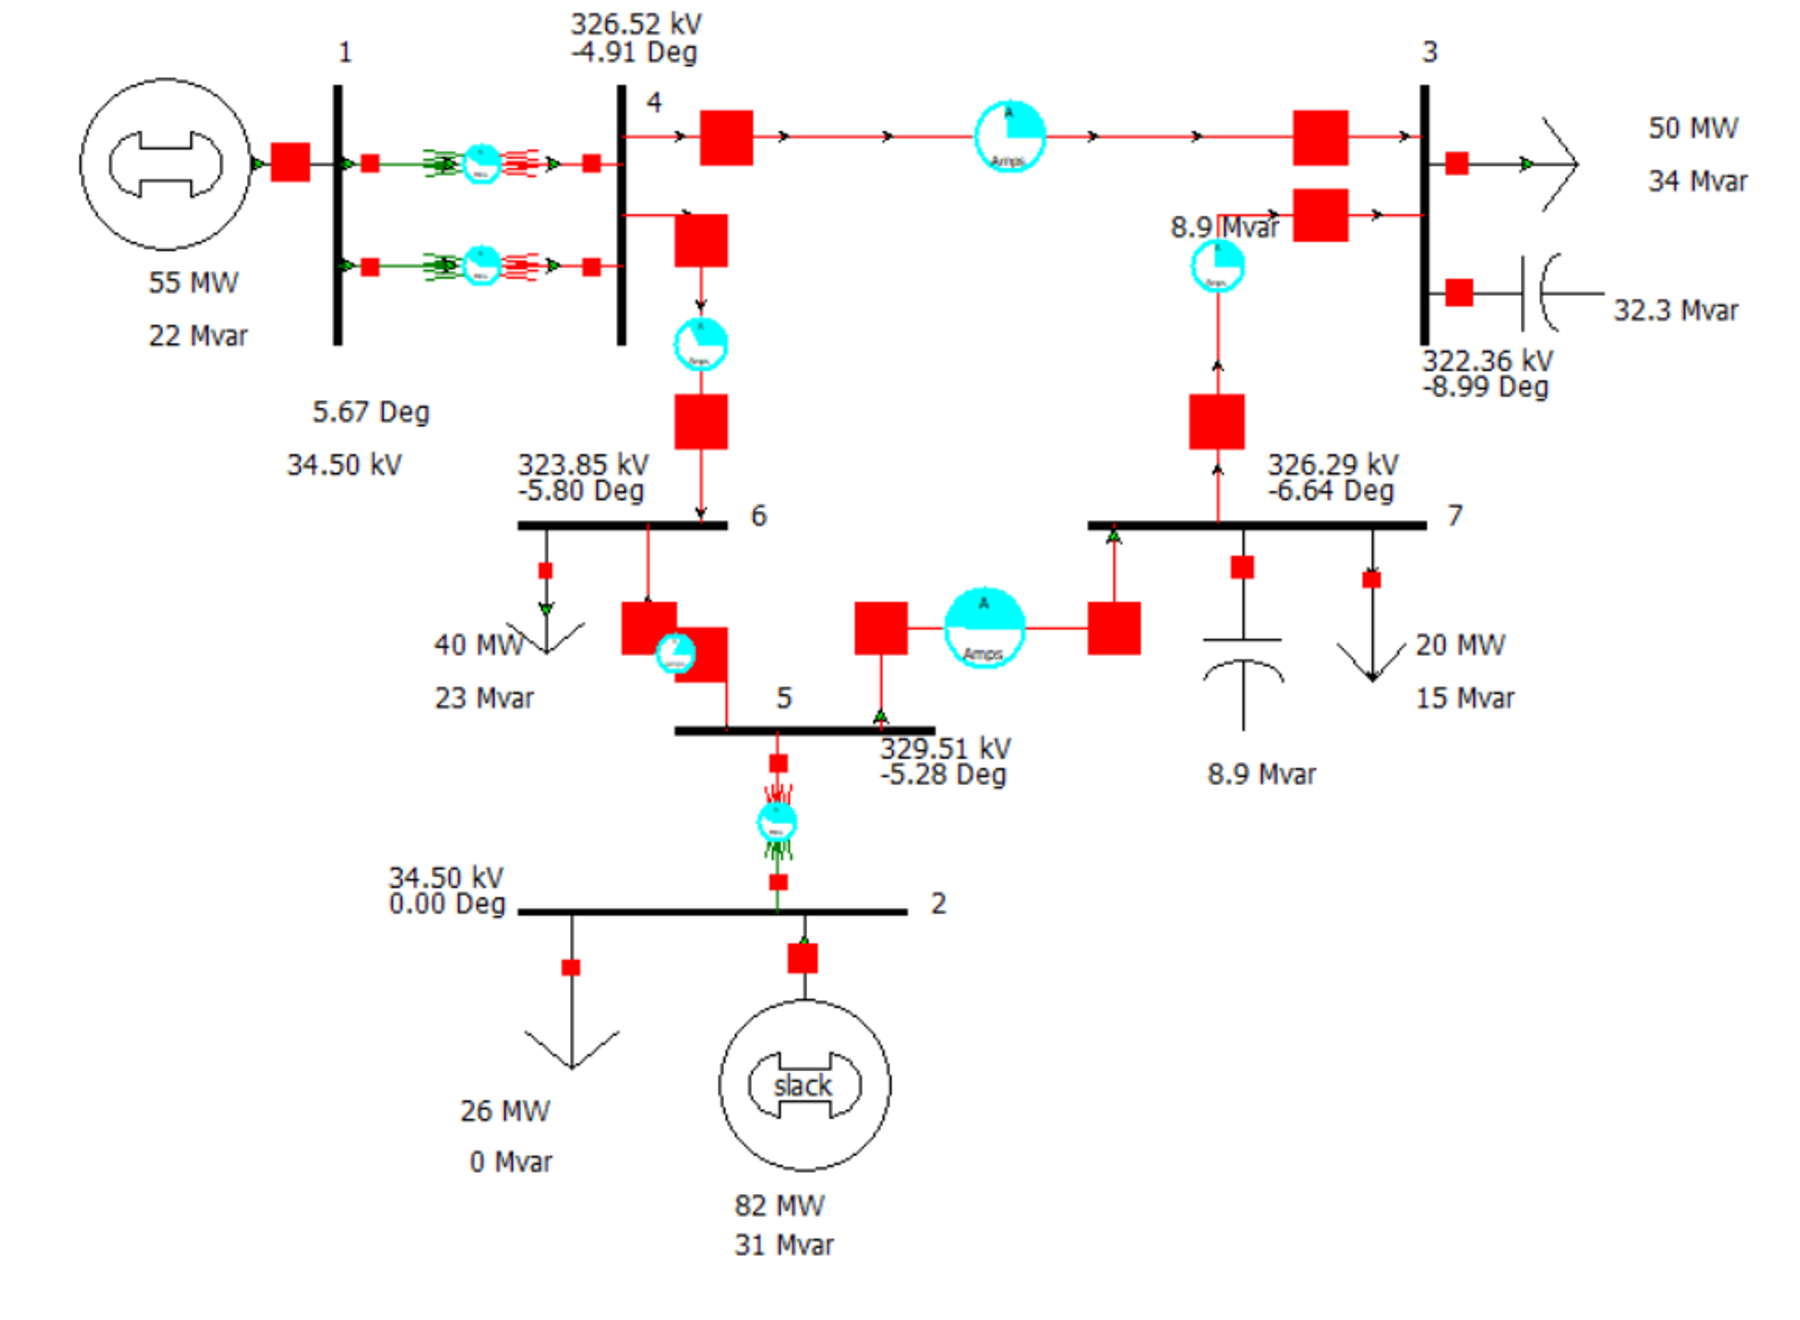
\includegraphics[width=\linewidth,height=.72\textheight,keepaspectratio]{assets/037_p017_01.png}\caption{Diagram or recorded result: Line outage and corrective load reduction.}\label{fig:037_p017_010}\end{figure}
\begin{figure}[!htbp]\centering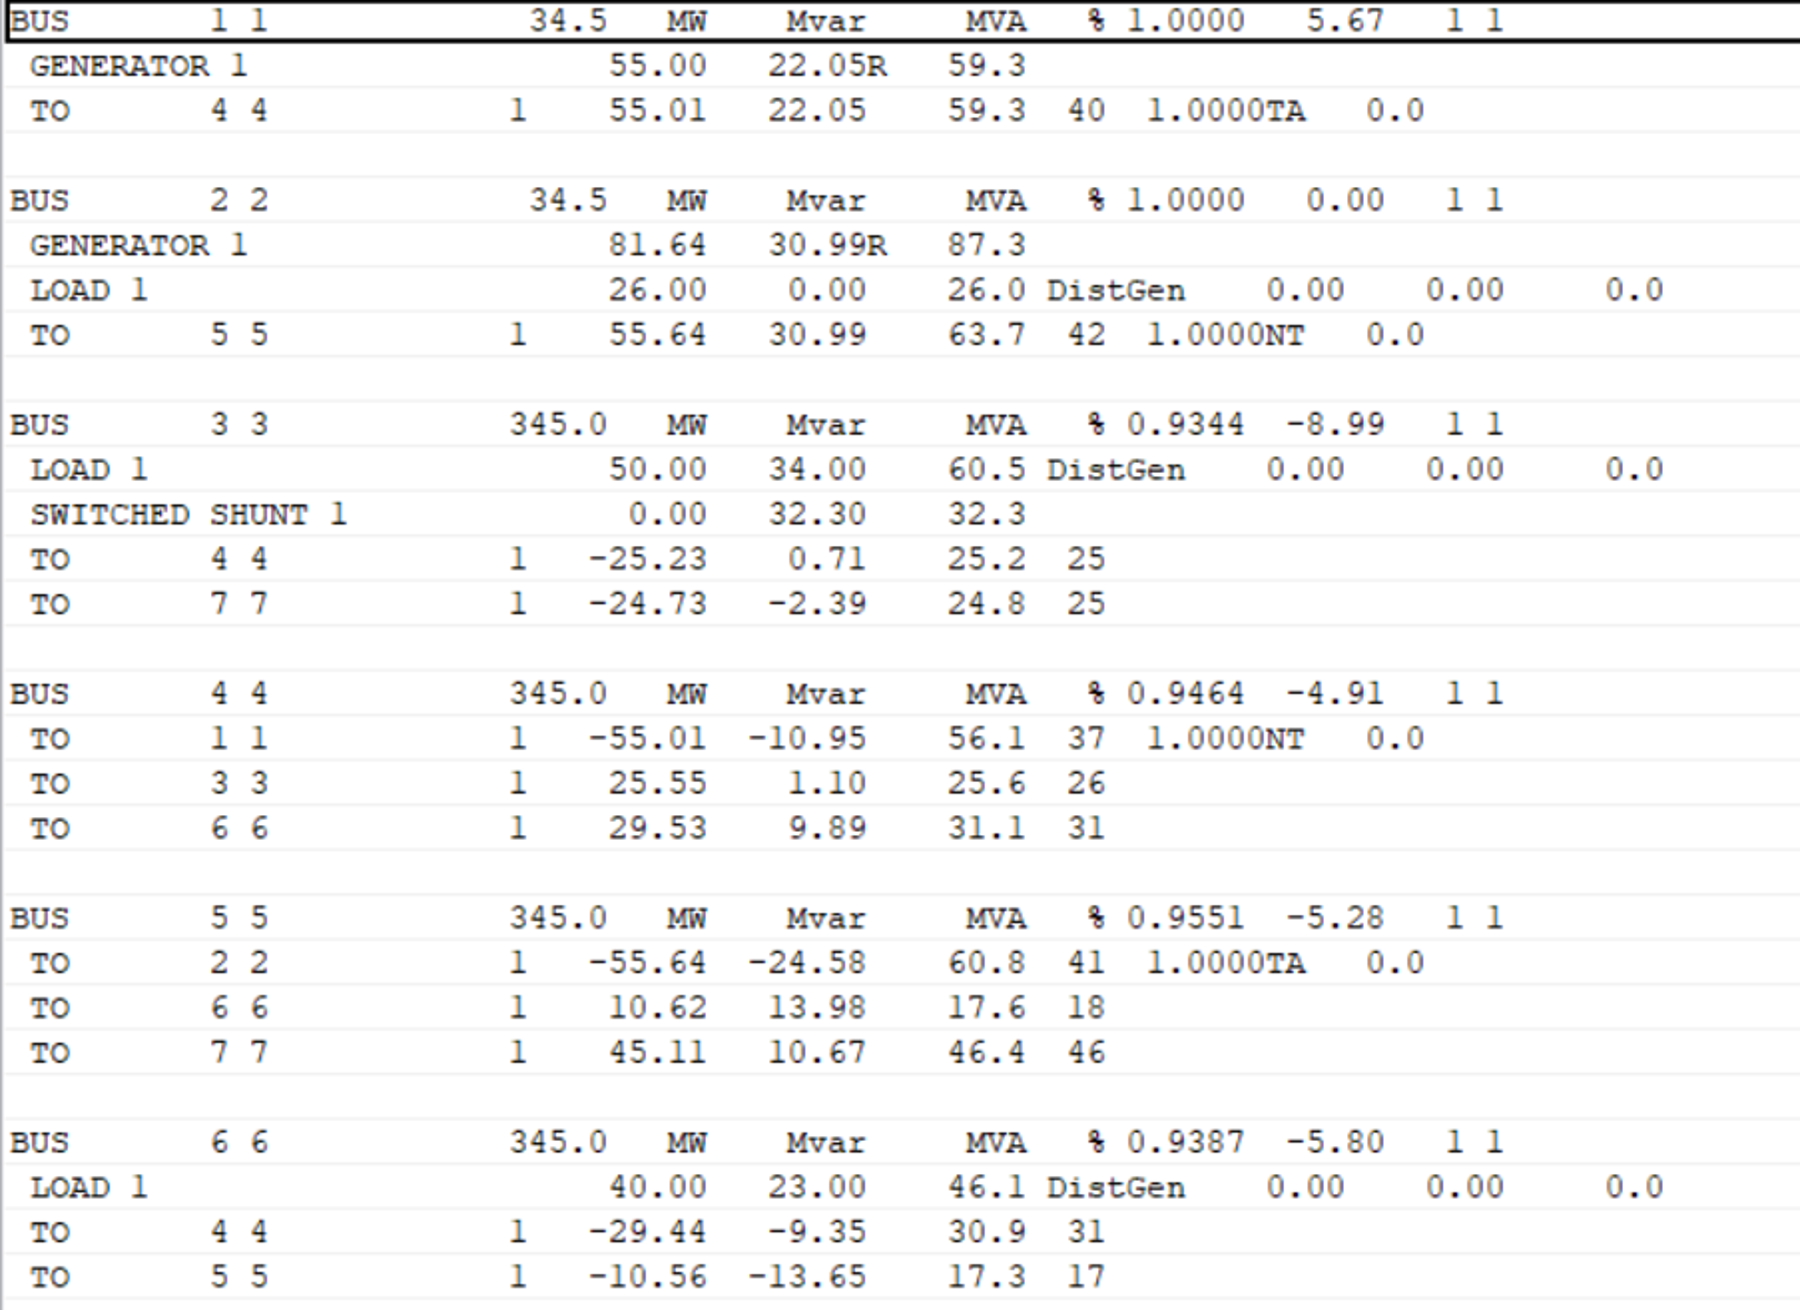
\includegraphics[width=\linewidth,height=.72\textheight,keepaspectratio]{assets/037_p017_02.png}\caption{Diagram or recorded result: Line outage and corrective load reduction.}\label{fig:037_p017_020}\end{figure}
\begin{figure}[!htbp]\centering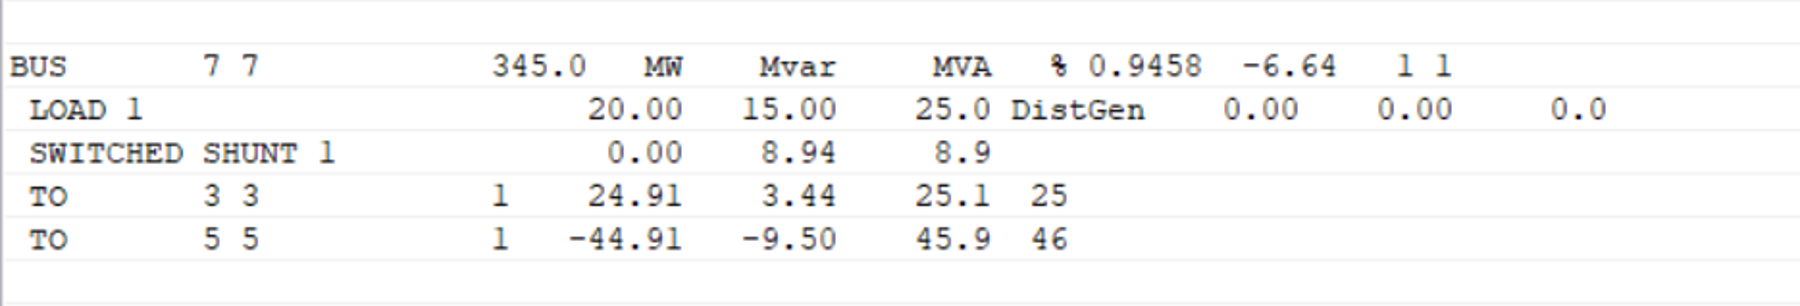
\includegraphics[width=\linewidth,height=.72\textheight,keepaspectratio]{assets/037_p017_03.png}\caption{Diagram or recorded result: Line outage and corrective load reduction.}\label{fig:037_p017_030}\end{figure}
\begin{figure}[!htbp]\centering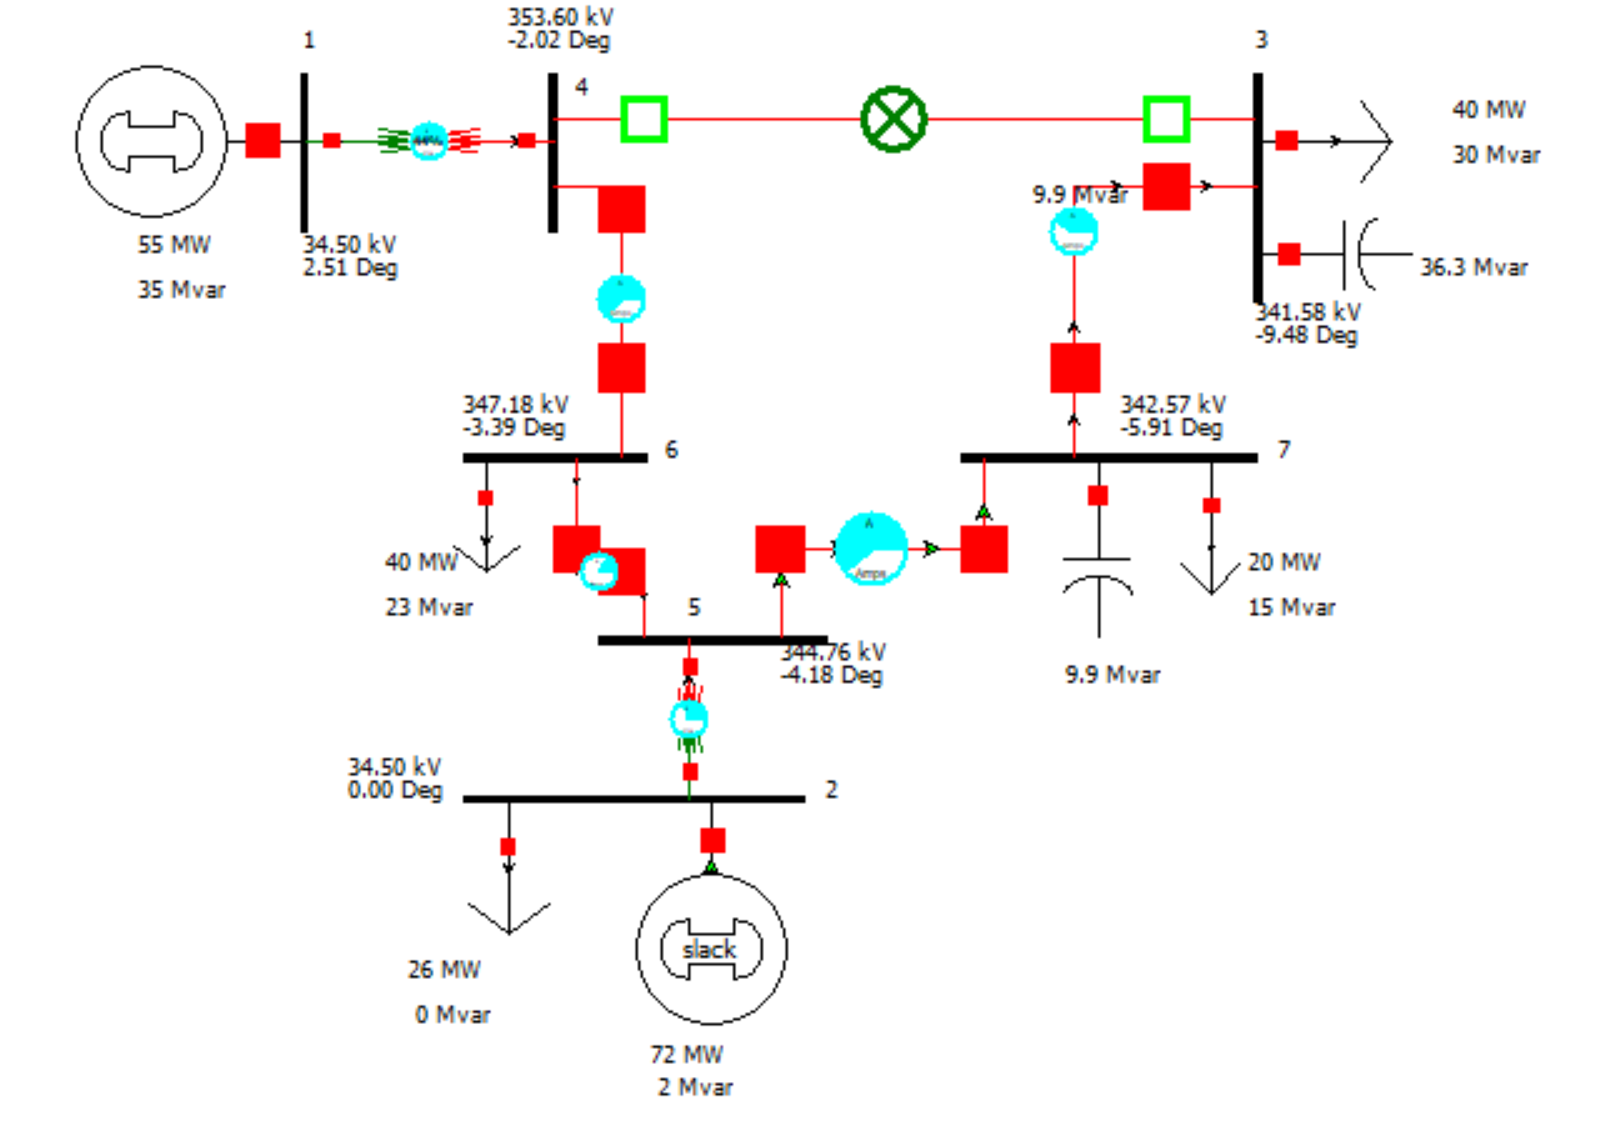
\includegraphics[width=\linewidth,height=.72\textheight,keepaspectratio]{assets/037_p018_01.png}\caption{Diagram or recorded result: Line outage and corrective load reduction.}\label{fig:037_p018_010}\end{figure}
\begin{figure}[!htbp]\centering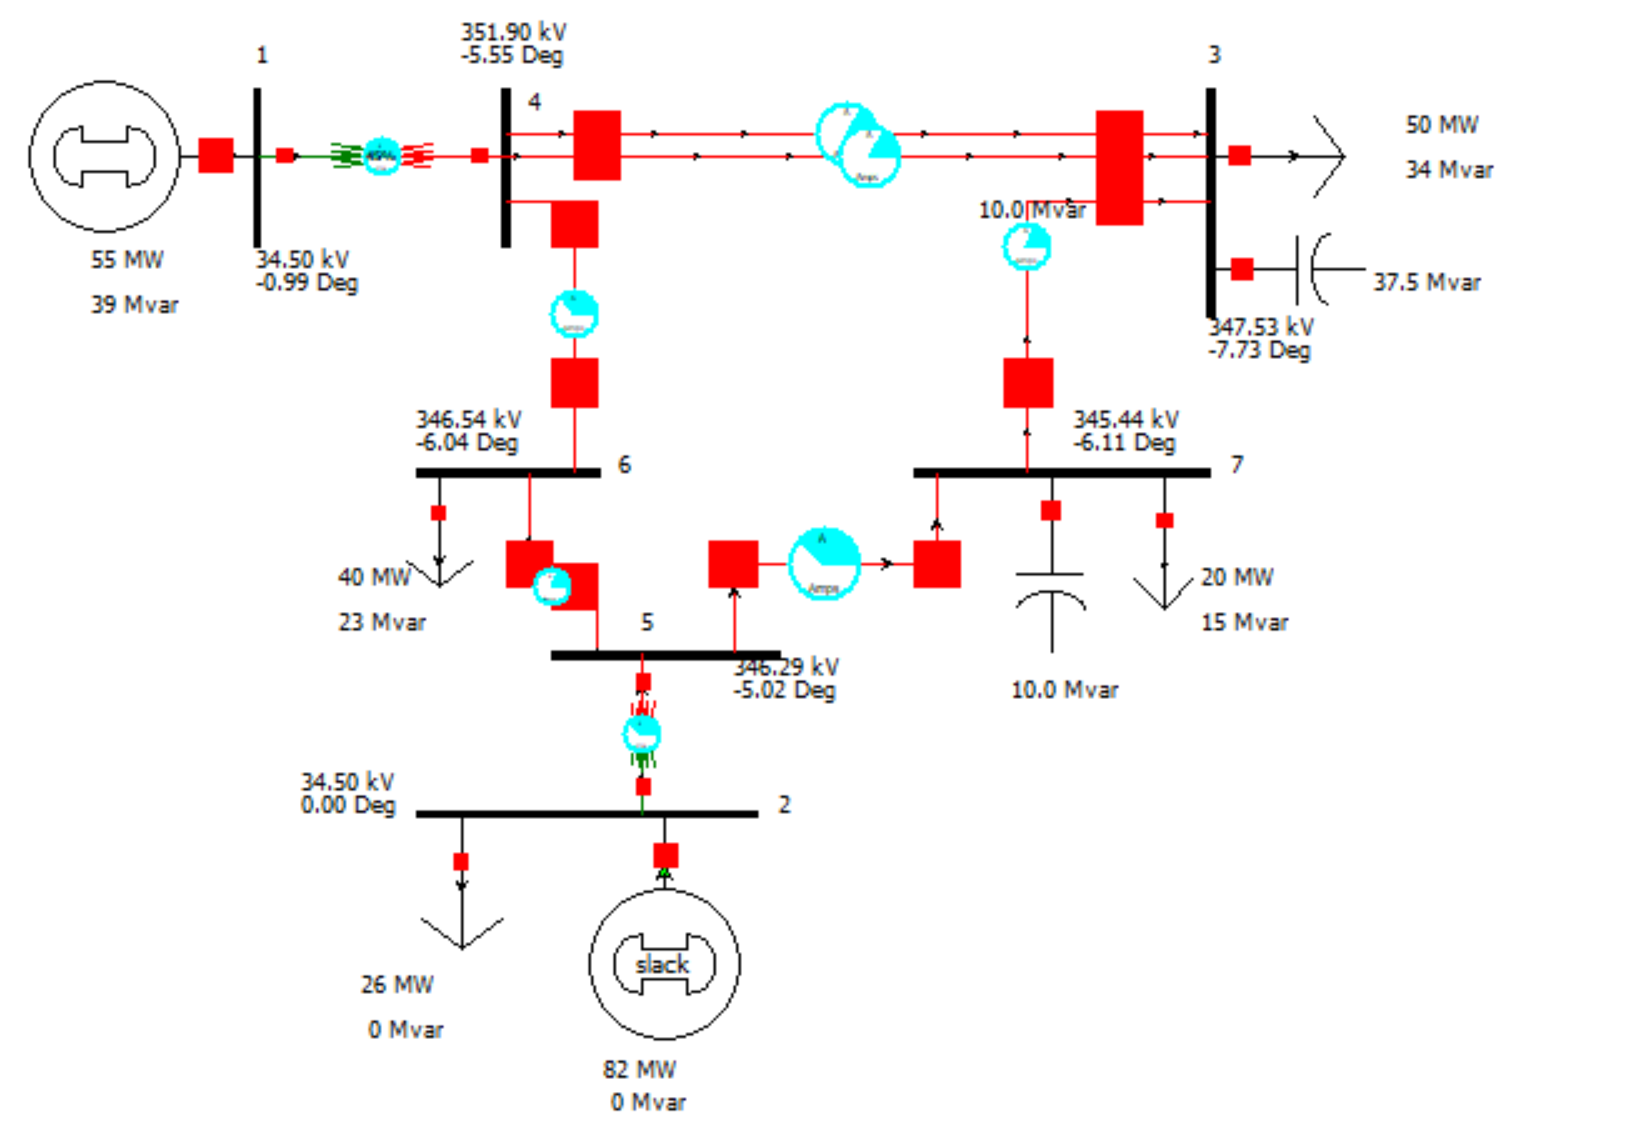
\includegraphics[width=\linewidth,height=.72\textheight,keepaspectratio]{assets/037_p019_01.png}\caption{Diagram or recorded result: Line outage and corrective load reduction.}\label{fig:037_p019_010}\end{figure}
\clearpage
\section{Parallel transmission line}

Adding an identical line between buses 3 and 4 yields before/\allowbreak{}after flow and total-loss views. The report observes smaller active and reactive losses. An additional path can reduce branch loading and effective transfer impedance, but actual improvement depends on the operating point, control response, and constraints. The retained tables show the submitted example;\allowbreak{} a general reliability claim needs contingency screening as well as the base-case comparison.

\begin{figure}[!htbp]\centering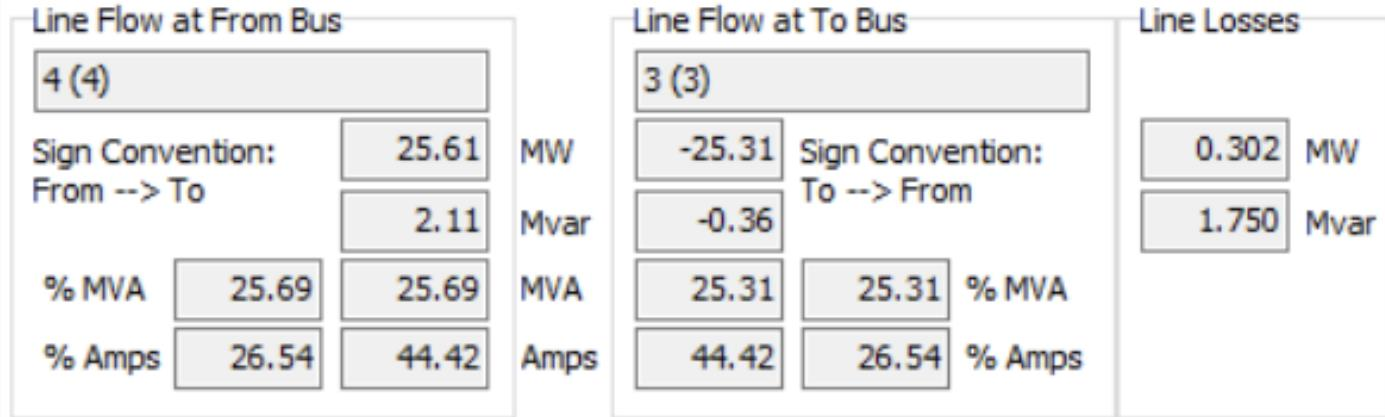
\includegraphics[width=\linewidth,height=.72\textheight,keepaspectratio]{assets/037_p020_01.png}\caption{Diagram or recorded result: Parallel transmission line.}\label{fig:037_p020_010}\end{figure}
\begin{figure}[!htbp]\centering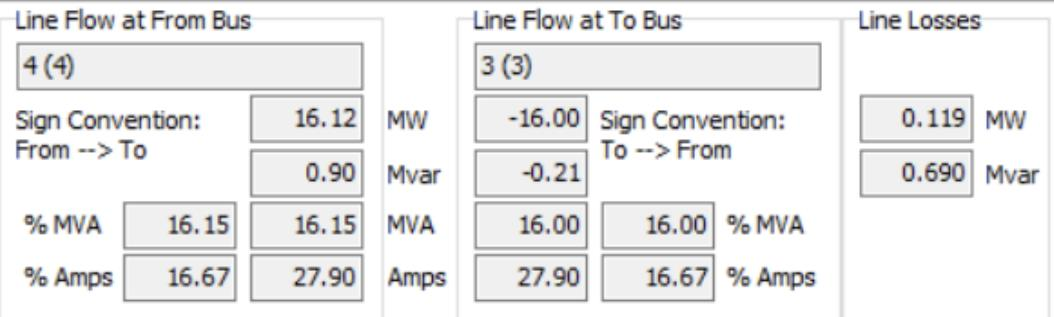
\includegraphics[width=\linewidth,height=.72\textheight,keepaspectratio]{assets/037_p020_02.png}\caption{Diagram or recorded result: Parallel transmission line.}\label{fig:037_p020_020}\end{figure}
\begin{figure}[!htbp]\centering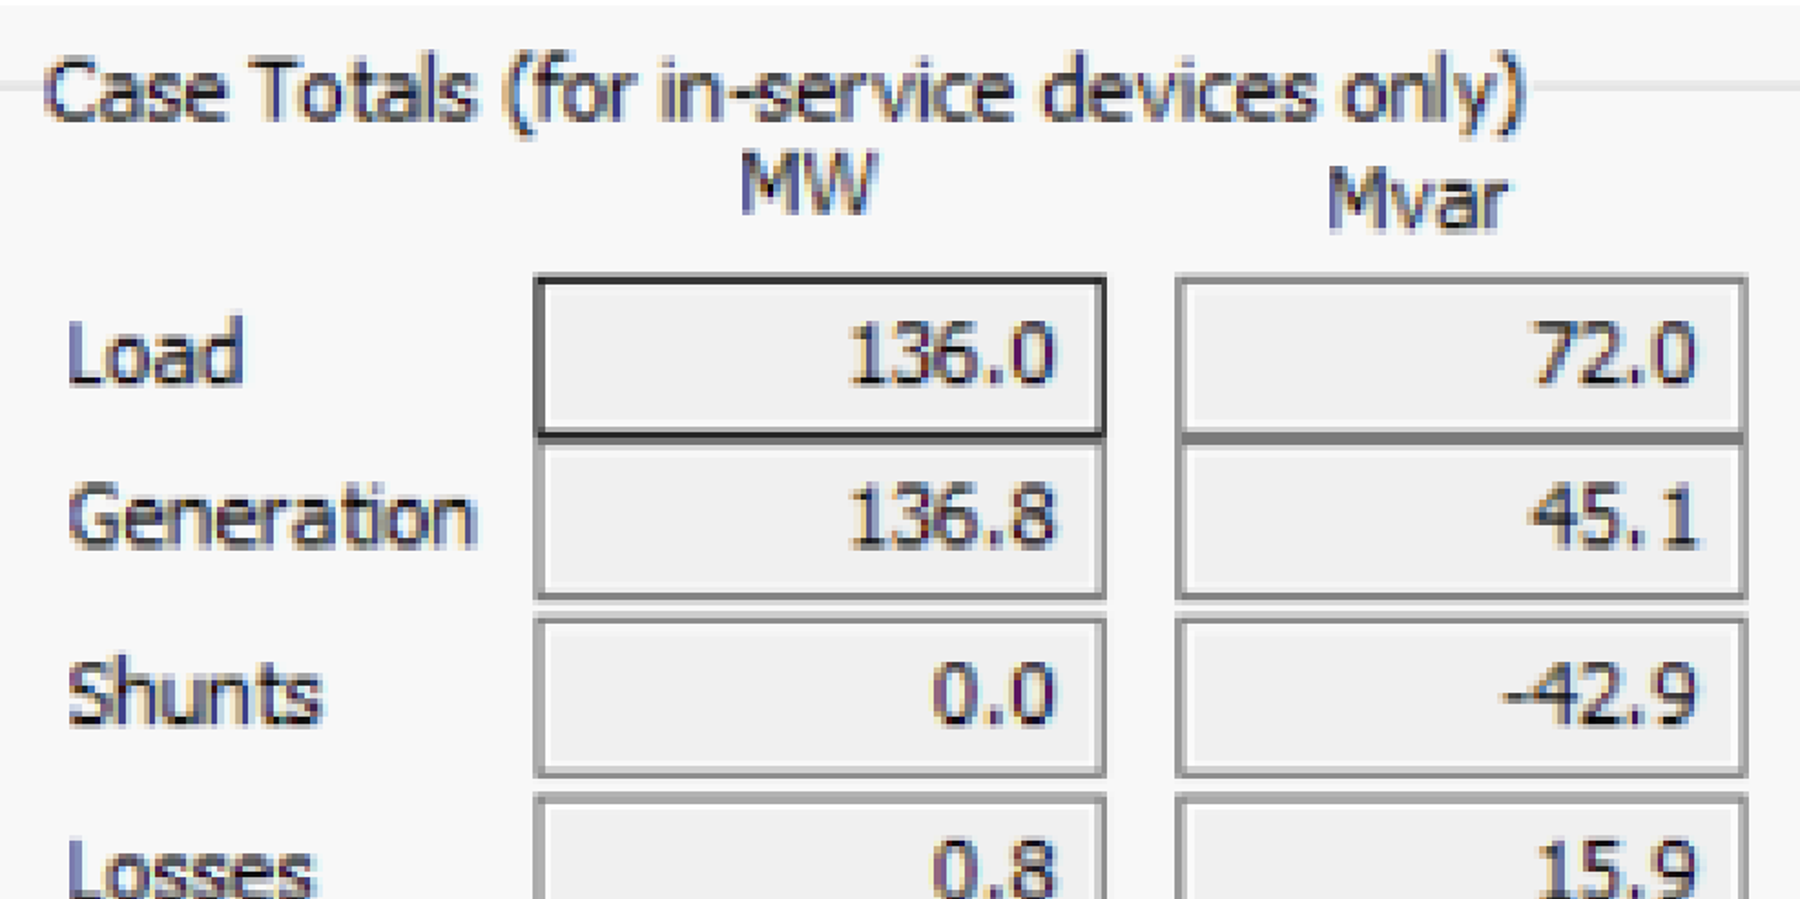
\includegraphics[width=\linewidth,height=.72\textheight,keepaspectratio]{assets/037_p021_01.png}\caption{Diagram or recorded result: Parallel transmission line.}\label{fig:037_p021_010}\end{figure}
\begin{figure}[!htbp]\centering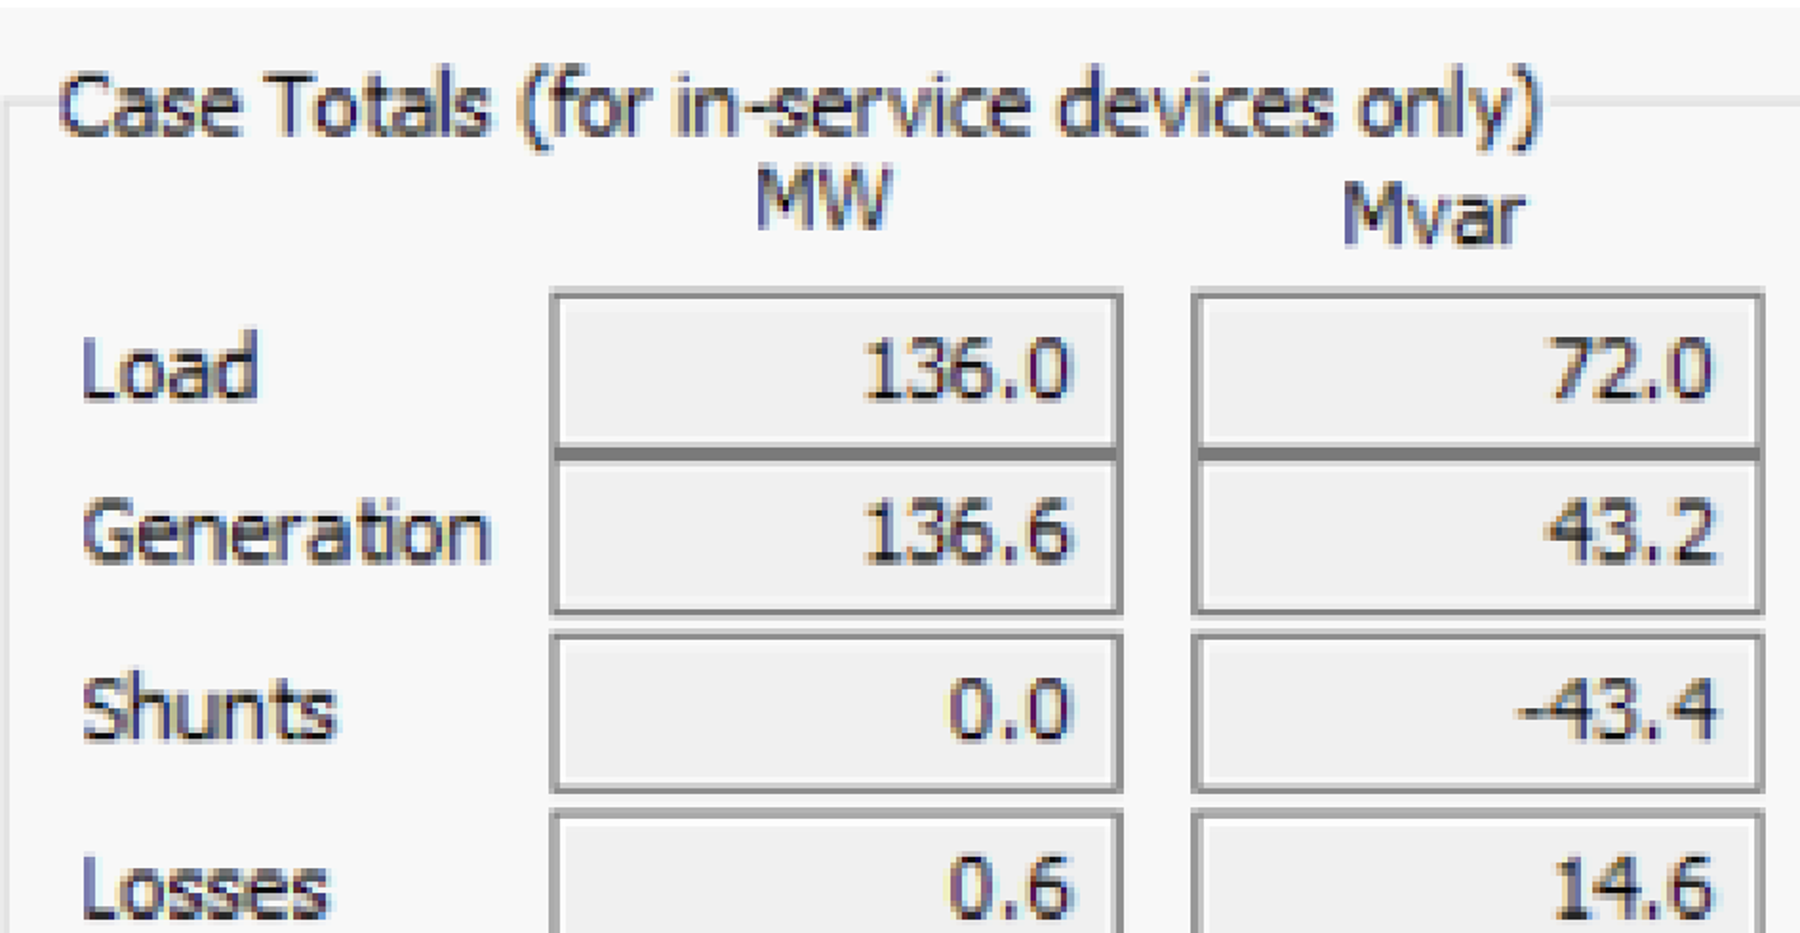
\includegraphics[width=\linewidth,height=.72\textheight,keepaspectratio]{assets/037_p021_02.png}\caption{Diagram or recorded result: Parallel transmission line.}\label{fig:037_p021_020}\end{figure}
\clearpage
\section{Contingency-analysis workflow and results}

The recorded workflow solves the base circuit, opens Tools/\allowbreak{}Contingency Analysis, inserts contingencies and actions, and selects Run. Its creation and result dialogs are preserved.


\begingroup\small\setlength{\tabcolsep}{3pt}\renewcommand{\arraystretch}{1.2}
\begin{longtable}{@{}p{0.3100\linewidth}p{0.3100\linewidth}p{0.3100\linewidth}@{}}
\toprule
\textbf{Contingency} & \textbf{Recorded outcome} & \textbf{Interpretation boundary} \\ \midrule
\endfirsthead
\textbf{Contingency} & \textbf{Recorded outcome} & \textbf{Interpretation boundary} \\ \midrule \endhead
Open line 3-4 & buses 3 and 7 below the stated lower voltage bound & steady-state voltage violation in the reported case \\
Open line 5-7 & solver does not converge to a displayed solution & investigate topology, controls, initialization, and feasibility;\allowbreak{} not a demonstrated dynamic-instability result \\
Move generator from bus 2 to bus 3 & no reported voltage-limit violation & limited to this modeled replacement and criterion \\
\bottomrule\end{longtable}\endgroup

Generator relocation is a comparison scenario, not ordinary immediate outage reserve unless a feasible replacement unit is actually available. Also check branch ratings, reactive limits, and island balance before declaring a case secure under broader criteria.

\begin{figure}[!htbp]\centering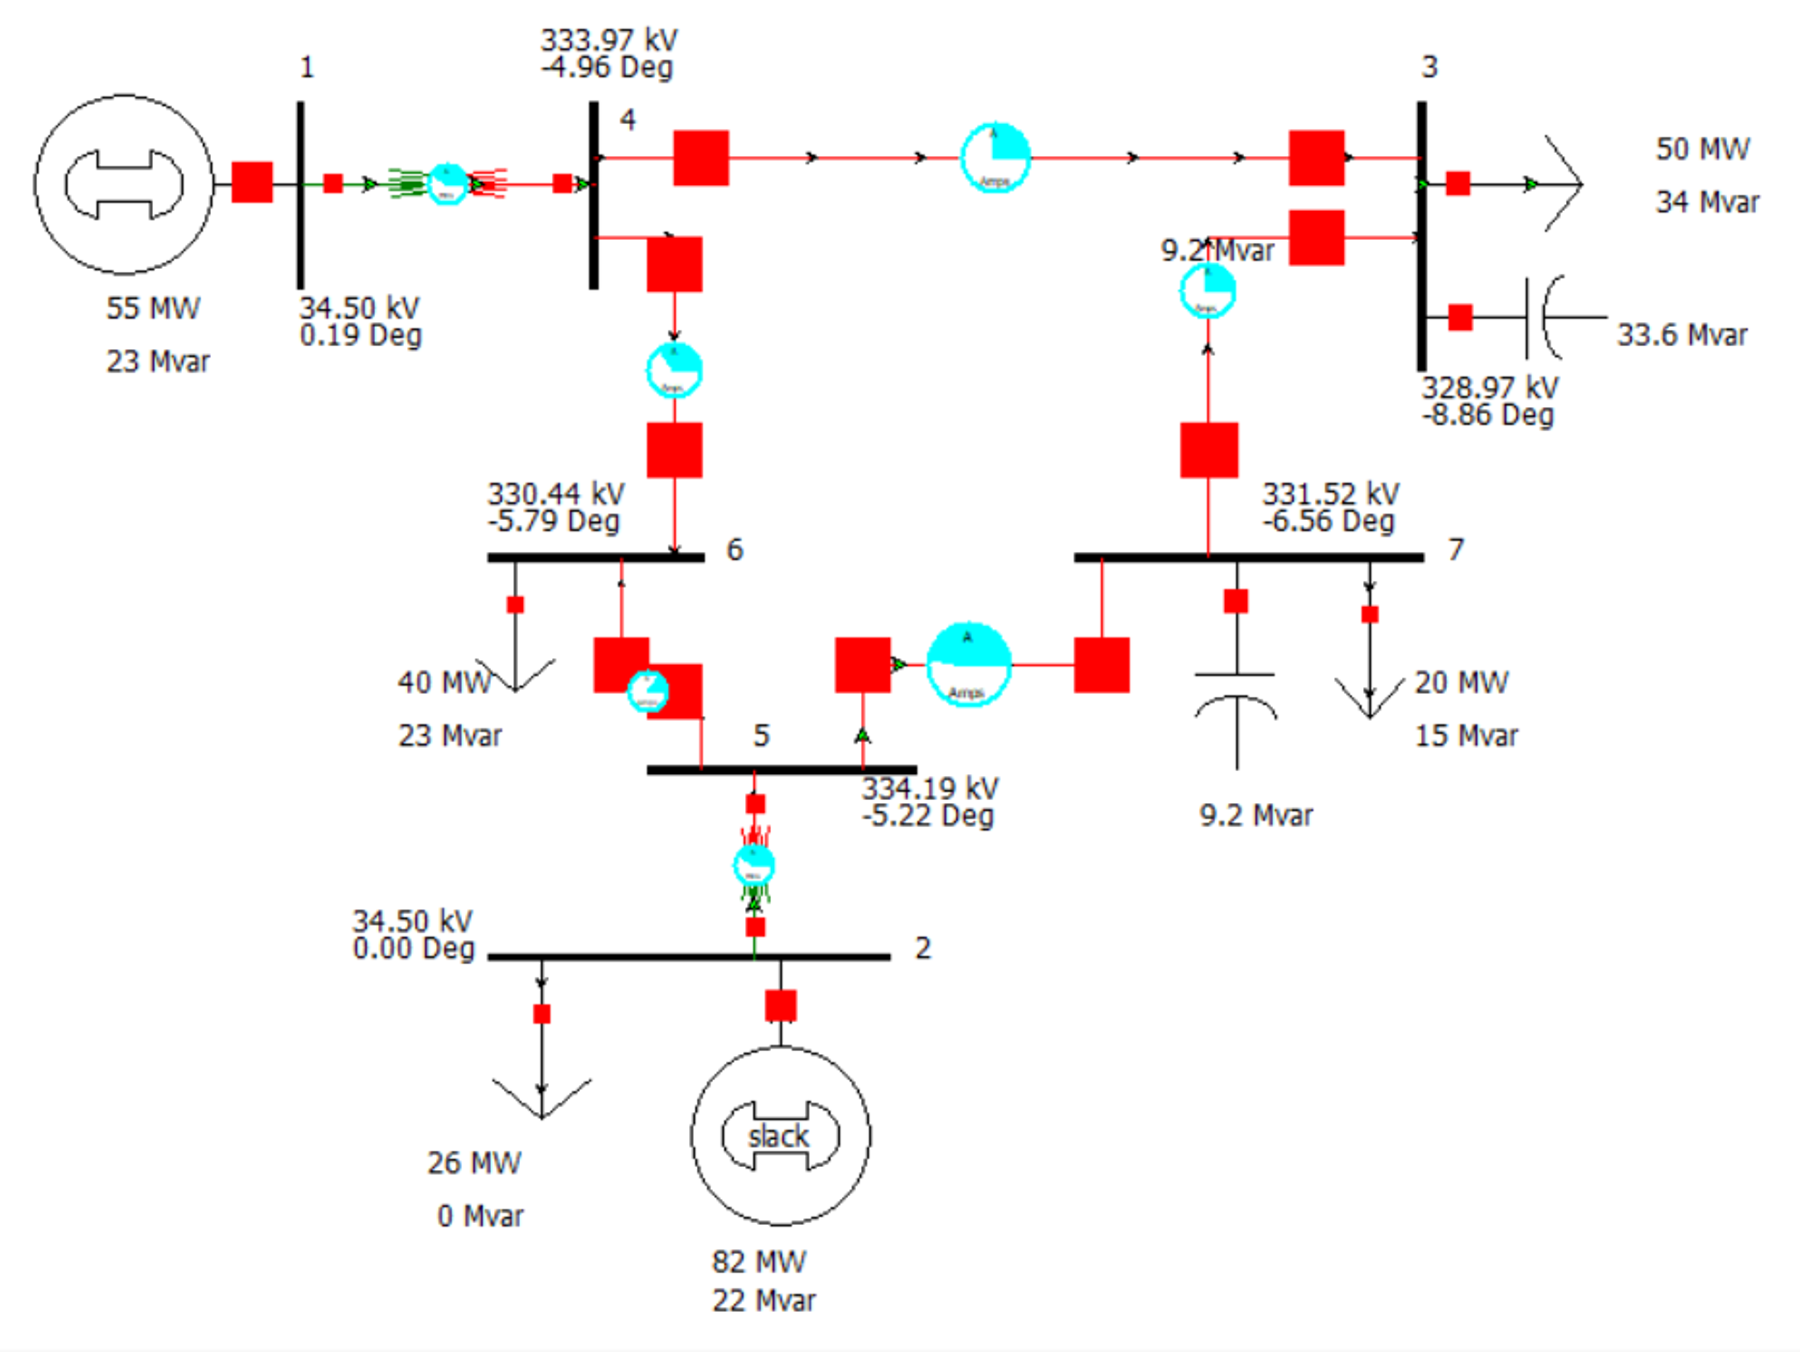
\includegraphics[width=\linewidth,height=.72\textheight,keepaspectratio]{assets/037_p022_01.png}\caption{Diagram or recorded result: Contingency-analysis workflow and results.}\label{fig:037_p022_010}\end{figure}
\begin{figure}[!htbp]\centering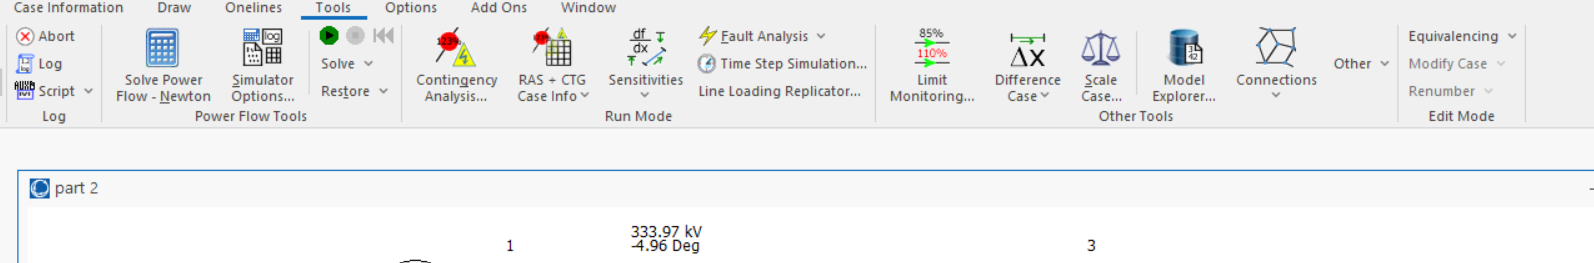
\includegraphics[width=\linewidth,height=.72\textheight,keepaspectratio]{assets/037_p023_01.png}\caption{Diagram or recorded result: Contingency-analysis workflow and results.}\label{fig:037_p023_010}\end{figure}
\begin{figure}[!htbp]\centering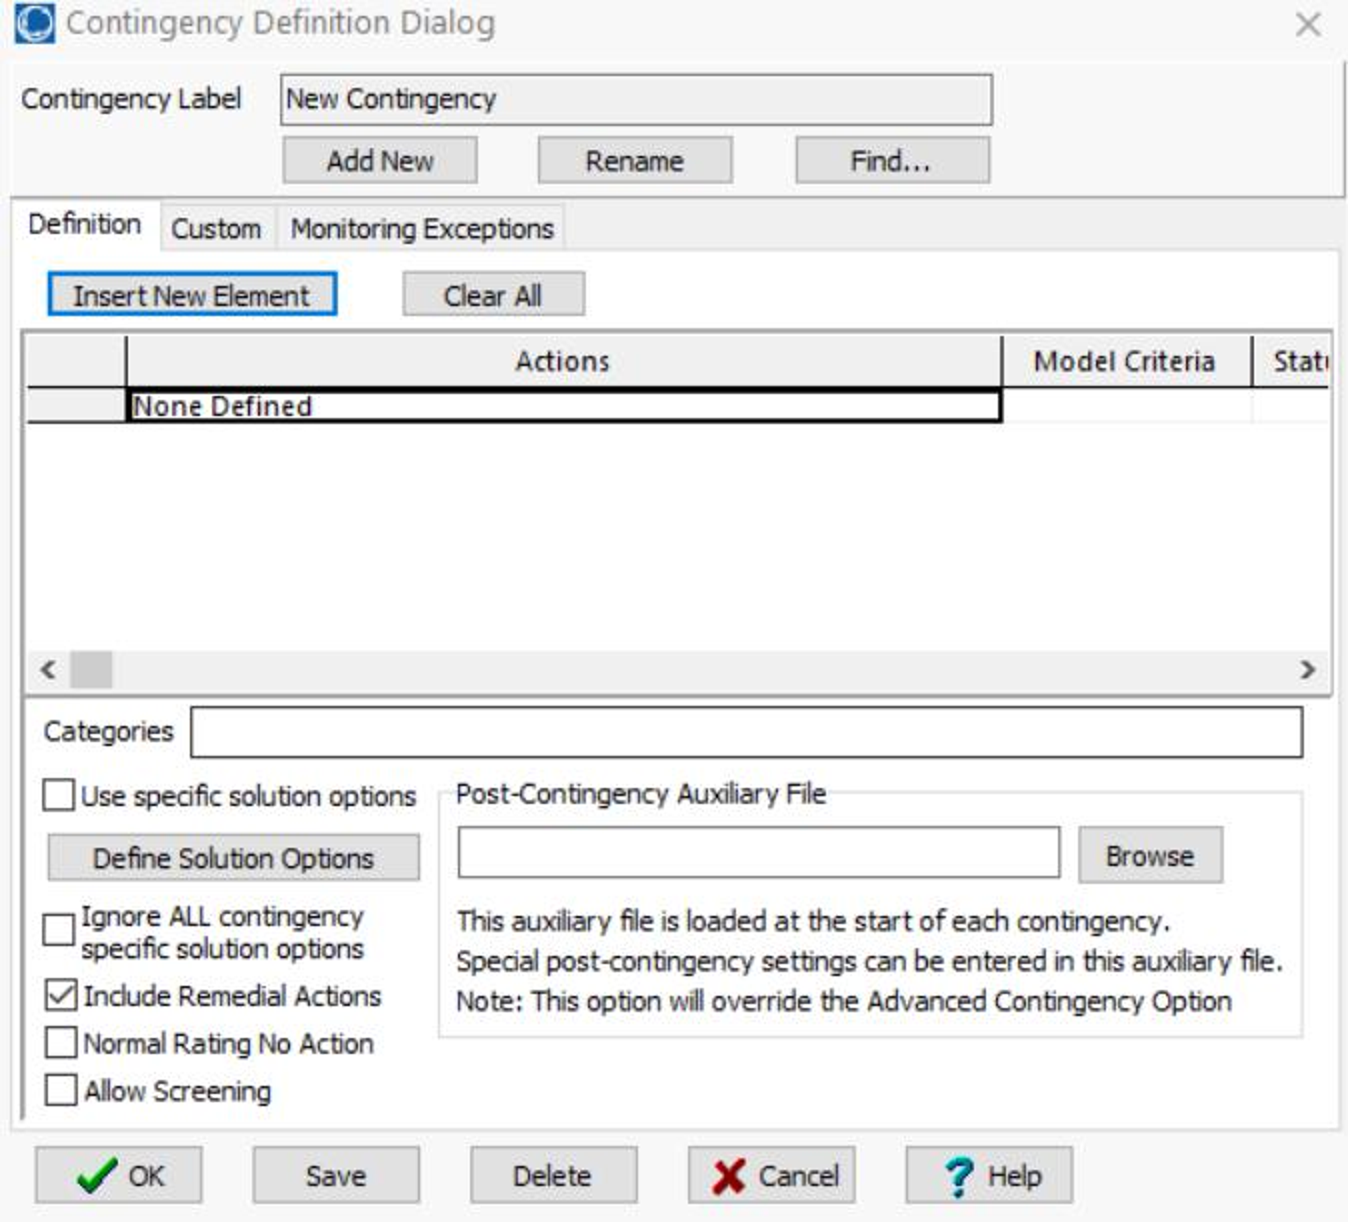
\includegraphics[width=\linewidth,height=.72\textheight,keepaspectratio]{assets/037_p023_02.png}\caption{Diagram or recorded result: Contingency-analysis workflow and results.}\label{fig:037_p023_020}\end{figure}
\clearpage
\section{Discussion: method selection}

Gauss-Seidel has a simple update and modest storage requirements. It can need many iterations and be sensitive to operating point and initialization. Newton-Raphson forms/\allowbreak{}factors a Jacobian and uses more work per step, but often converges in fewer steps. The report prefers Newton for larger networks. Avoid claiming inherently higher final accuracy when both methods satisfy the same residual tolerance.

\begin{figure}[!htbp]\centering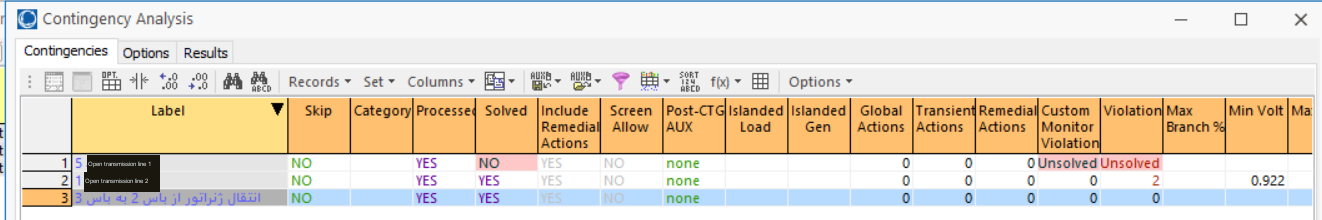
\includegraphics[width=\linewidth,height=.72\textheight,keepaspectratio]{assets/037_p024_01.png}\caption{Diagram or recorded result: Discussion: method selection.}\label{fig:037_p024_010}\end{figure}
\begin{figure}[!htbp]\centering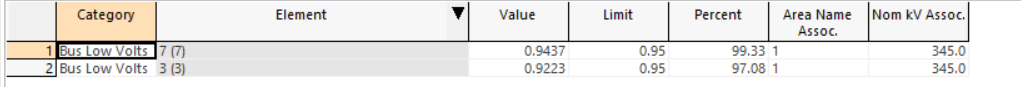
\includegraphics[width=\linewidth,height=.72\textheight,keepaspectratio]{assets/037_p024_02.png}\caption{Diagram or recorded result: Discussion: method selection.}\label{fig:037_p024_020}\end{figure}
\begin{figure}[!htbp]\centering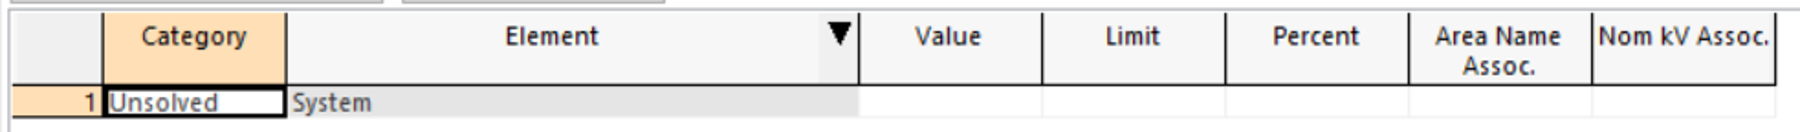
\includegraphics[width=\linewidth,height=.72\textheight,keepaspectratio]{assets/037_p024_03.png}\caption{Diagram or recorded result: Discussion: method selection.}\label{fig:037_p024_030}\end{figure}
\begin{figure}[!htbp]\centering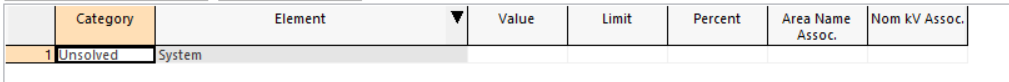
\includegraphics[width=\linewidth,height=.72\textheight,keepaspectratio]{assets/037_p024_04.png}\caption{Diagram or recorded result: Discussion: method selection.}\label{fig:037_p024_040}\end{figure}
\clearpage
\section{Discussion: compensation, OPF data, and resilience}

Shunt banks supply reactive power locally, supporting voltage and reducing reactive transfer where appropriately sized. Their location, switching, voltage limits, and resonance/\allowbreak{}control interactions matter. The supplied case demonstrates particular voltage/\allowbreak{}loss effects rather than a complete compensation design. OPF requires topology and impedances;\allowbreak{} generator capabilities and active/\allowbreak{}reactive limits;\allowbreak{} load data;\allowbreak{} voltage and branch constraints;\allowbreak{} transformer controls;\allowbreak{} objective/\allowbreak{}cost functions;\allowbreak{} and a specified dispatch policy. Startup costs and ramp limits belong to formulations that explicitly model commitment or time coupling, rather than every static OPF. The report proposes reserve generation, stronger/\allowbreak{}parallel transmission paths, suitable transformers, capacitor banks, and smarter protection. These can contribute to resilience, but their benefit needs scenario-specific study and coordination. Proposed protective systems and reserve plants were not implemented in this project. The source case files and outputs are organized separately to support later reproduction in PowerWorld.

\end{document}